\chapter{Release 1 : sprint1, sprint2 et sprint3}


\section{Introduction}

Cette première release constitue la base fondamentale du système en regroupant les \textit{Sprint 1}, \textit{Sprint 2} et \textit{Sprint 3}. Elle couvre la gestion des accès et des entités organisationnelles, la configuration du catalogue de services administratifs ainsi que la dématérialisation complète des demandes des citoyens. Cette release jette les fondations techniques et fonctionnelles du système et marque le passage d’une infrastructure sécurisée vers une plateforme pleinement opérationnelle orientée utilisateur.


\section{Sprint 1 : Socle d'accès et structures institutionnelles}

Le premier sprint vise principalement à mettre en place les fondations de la plateforme, notamment la gestion des utilisateurs, l’authentification, l’autorisation ainsi que la structuration des entités administratives et institutionnelles.


\subsection{Backlog du Sprint 1}

Nous proposons, à travers le tableau~\ref{tab:user-stories-sprint1} une présentation détaillée du backlog du sprint 1, accompagnée des estimations en jours de chaque tâche.



\renewcommand{\arraystretch}{1.3}

\begin{longtable}{|p{1cm}|p{3cm}|p{7cm}|p{1cm}|p{2cm}|}

\hline
\rowcolor{orange!30}
\textbf{ID} & \textbf{En tant que} & \textbf{User Story} & \textbf{Est/J} & \textbf{Priorité} \\
\hline
\endfirsthead



US1 & Administrateur &
Je veux m’authentifier afin d’accéder au backoffice &
2 & Élevée \\ \hline

US2 & Administrateur système &
Je veux gérer les comptes des administrateurs backoffice afin de contrôler l’accès au système &
4 & Élevée \\ \hline

US3 & Administrateur système &
Je veux gérer les rôles afin de définir les niveaux d’accès des utilisateurs &
2 & Élevée \\ \hline

US4 & Administrateur système &
Je veux consulter les permissions afin de contrôler les actions autorisées &
1 & Élevée \\ \hline

US8 & Administrateur &
Je veux modifier mon profil afin de mettre à jour mes informations &
1 & Moyenne \\ \hline

US5 & Administrateur ministériel &
Je veux gérer les comptes des administrateurs institutionnels afin d’assurer leur accès et leurs droits &
4 & Élevée \\ \hline

US6 & Administrateur système &
Je veux gérer les administrations ministérielles afin d’organiser les structures &
4 & Élevée \\ \hline

US7 & Administrateur système &
Je veux gérer les langues de la plateforme afin de garantir une interface multilingue &
2 & Élevée \\ \hline

\caption{Backlog du Sprint 1}
\label{tab:user-stories-sprint1}

\end{longtable}





\subsection{Diagramme de cas d’utilisation du sprint 1}

Le diagramme de cas d'utilisation du sprint 1 est présenté dans la figure \ref{fig:cas-utilisation-sprint1}.


\begin{figure}[H]
    \centering
    \includegraphics[width=16cm,height=16cm]{images/diagrammes/sprint1/cas-utili-sprin1.drawio.png}
    \caption{Diagramme de cas d’utilisation -- Sprint 1}
    \label{fig:cas-utilisation-sprint1}
\end{figure}

\subsection{Diagramme de classe du sprint 1}

La figure \ref{fig:cas-utilisation-classe} présente le diagramme de classe du sprint 1.
 
\begin{figure}[H]
    \centering
    \includegraphics[width=16cm,height=16cm]{images/diagrammes/sprint1/diag-classe-sprint1.drawio.png}
    \caption{Diagramme de classe -- Sprint 1}
    \label{fig:cas-utilisation-classe}
\end{figure}


\subsection{Raffinement et description textuelle du cas d'utilisation «Gérer les administrations»}

Dans cette section, nous utiliserons le diagramme raffiné et les descriptions de scénarios pour décrire le cas « Gérer les administrations». Ce dernier montre les sous-opérations
possibles à faire.

La figure \ref{fig:cas-utilisation-raffiné-gérer-administrations}  représente le diagramme de cas d'utilisation raffiné du cas d'utilisation « Gérer les administrations ».

\begin{figure}[H]
    \centering
    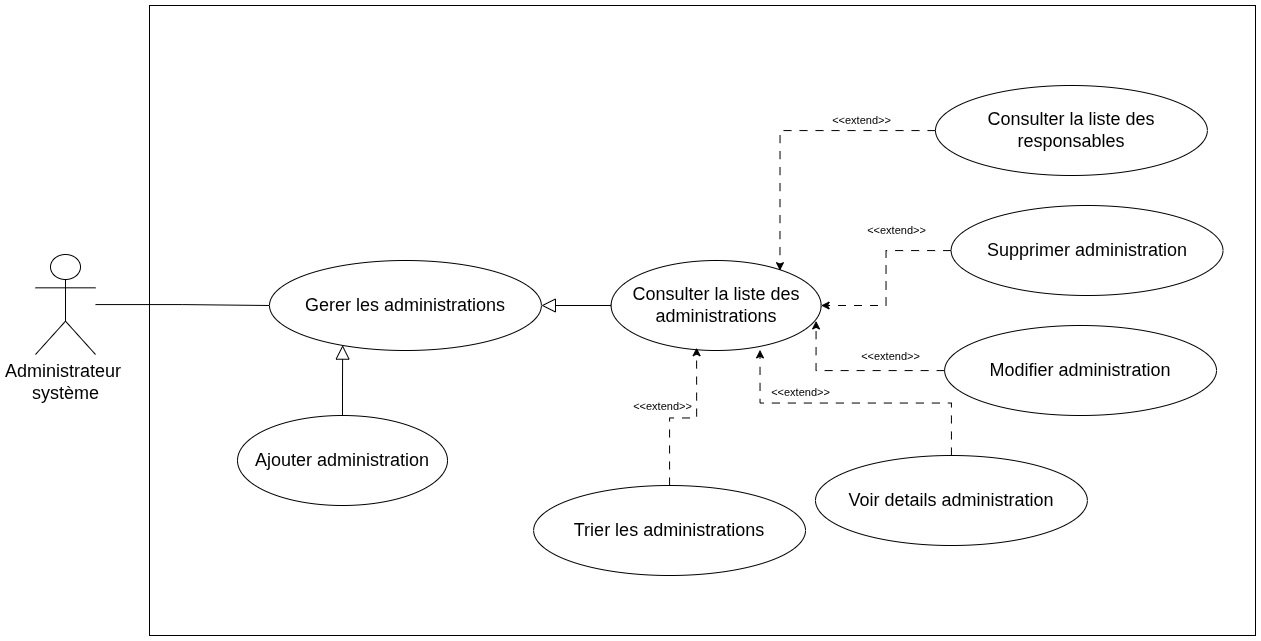
\includegraphics[width=17cm,height=9cm]{images/diagrammes/sprint1/cas-utilisation-gerer-administration.png}
    \caption{Raffinement du cas d'utilisation « Gérer les administrations »}
    \label{fig:cas-utilisation-raffiné-gérer-administrations}
\end{figure}

\textbf{Description textuelle}

Une description des scénarios du cas "Ajouter une administration" est présentée dans le tableau~\ref{tab:ajouter-admin}.

\renewcommand{\arraystretch}{1.3}

\begin{longtable}{|p{4cm}|p{12cm}|}
\hline

\rowcolor{gray!20}
\textbf{Champ} & \textbf{Description} \\ \hline
\endfirsthead

 
Nom & Ajouter une administration \\ \hline

Acteur principal & Administrateur système \\ \hline

Objectif & Permettre à l’administrateur de créer une nouvelle administration ministérielle dans le système afin de structurer l’organisation administrative. \\ \hline

Pré-condition &
\begin{itemize}
    \item L’administrateur est identifié.
    \item L'administrateur possède les droits requis.
\end{itemize}
\\ \hline

Scénario nominal &
\begin{enumerate}
    \item L’administrateur accède au module de gestion des administrations.
    \item Il clique sur l’option "Ajouter une administration".
    \item Le système présente le formulaire de création.
    \item L’administrateur renseigne les informations nécessaires (nom, responsable, coordonnées, etc.).
    \item L'administrateur vérifie le formulaire.
    \item Le système vérifie que les données saisies sont valides.
    \item Le système enregistre la nouvelle gestion.
    \item Le système affiche un message de confirmation.
\end{enumerate}
\\ \hline

Scénario alternatif &
\begin{itemize}
    \item Si les données saisies sont invalides ou incomplètes, le système affiche un message d’erreur.
\end{itemize}
\\ \hline

\caption{Description textuelle - Ajouter une administration}
\label{tab:ajouter-admin}
\end{longtable}


Une description du cas "Supprimer une administration" est présentée dans le tableau~\ref{tab:supprimer-admin}.
\renewcommand{\arraystretch}{1.3}

\begin{longtable}{|p{4cm}|p{12cm}|}
\hline

\rowcolor{gray!20}
\textbf{Champ} & \textbf{Description} \\ \hline
\endfirsthead

 

Nom & Supprimer une administration \\ \hline

Acteur principal & Administrateur système \\ \hline

Objectif & Permettre à l’administrateur de supprimer une administration existante du système. \\ \hline

Pré-condition &
\begin{itemize}
    \item L’administrateur est identifié.
    \item L’administration existe dans le système.
    \item L'administrateur possède les droits requis.
\end{itemize}
\\ \hline

Scénario nominal &
\begin{enumerate}
    \item L'administrateur peut consulter la liste des organismes gouvernementaux.
    \item Il sélectionne une administration.
    \item Il clique sur l’option "Supprimer".
    \item Le système sollicite une confirmation.
    \item L’administrateur valide la suppression.
    \item Le système fait disparaître l’administration.
    \item Un message de confirmation s’affiche sur le système.
\end{enumerate}
\\ \hline

Scénario alternatif &
\begin{itemize}
    \item Si l’administration est liée à des données (services, agents), le système empêche la suppression.
    \item Si l’administrateur annule l’action, aucune modification n’est effectuée.
    \item En cas d’erreur système, un message d’échec est affiché.
\end{itemize}
\\ \hline

\caption{Description textuelle - Supprimer une administration}
\label{tab:supprimer-admin}
\end{longtable}


\subsection{Les diagrammes de séquences du cas d’utilisation « Gérer les administrations »}

Nous avons choisi, dans cette section d’illustrer uniquement certains diagrammes de séquence parmi ceux définis lors de l’étape de raffinement. Ce choix a été fait pour mettre en avant les interactions les plus importantes dans le cas d’usage « Gérer les administrations », dont les opérations principales telles que l’ajout et la suppression d’une administration.

\noindent  \textbf{Présentation des diagrammes de séquences :}

Ce diagramme illustre le processus d’ajout d’une nouvelle administration depuis la saisie des informations par l’utilisateur jusqu’à leur enregistrement dans le système comme présenté dans la figure~\ref{fig:ajouter-administration}.


\begin{figure}[H]
    \centering
    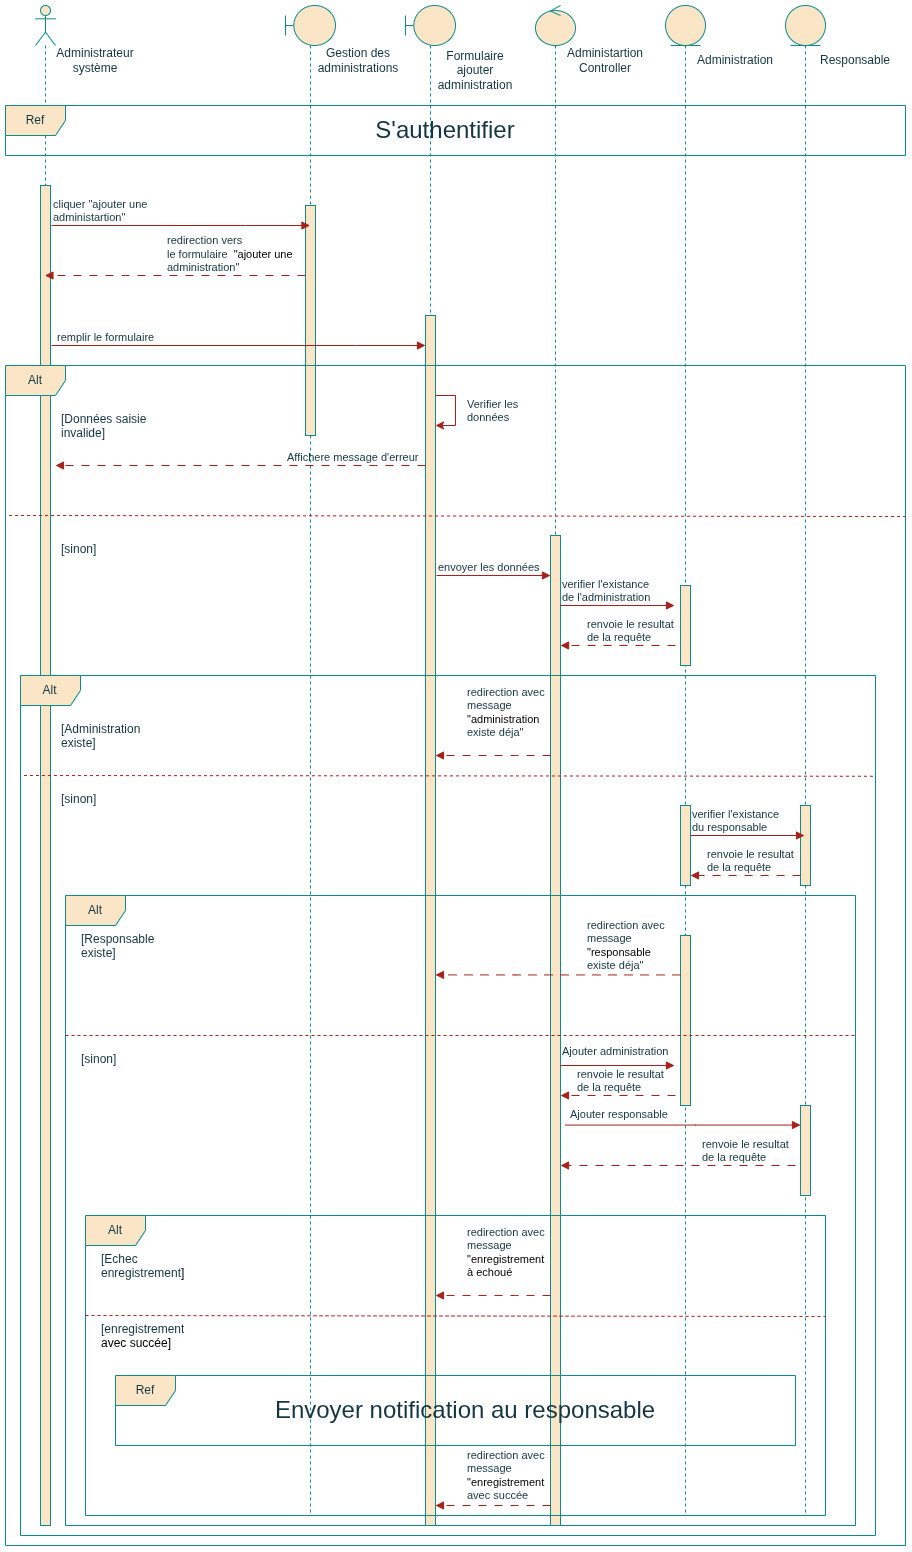
\includegraphics[width=15cm,height=22cm]{images/diagrammes/sprint1/vrai-ajouter-administration.drawio.png}
    \caption{Diagramme de séquence - Ajouter une administration}
    \label{fig:ajouter-administration}
\end{figure}

% Supprimer
Ce diagramme décrit le processus de suppression d’une administration, incluant la confirmation de l’action et la suppression définitive des données, comme illustré dans la figure~\ref{fig:supprimer-administration}.


\begin{figure}[H]
    \centering
    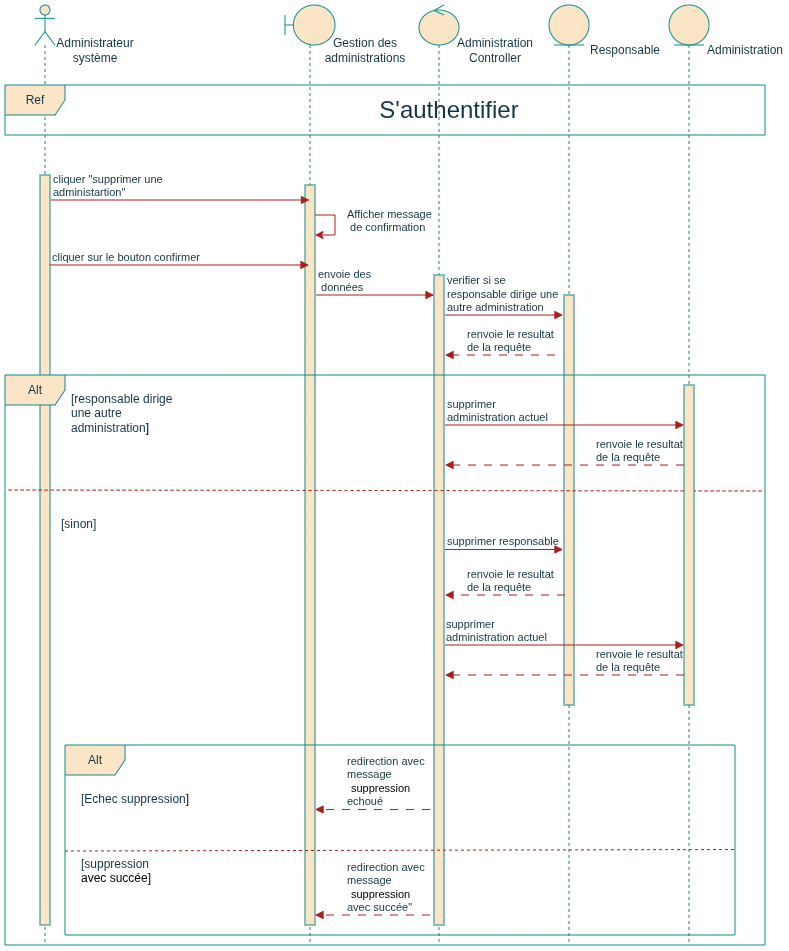
\includegraphics[width=15cm,height=19cm]{images/diagrammes/sprint1/vrai-supp-administration.drawio.png}
    \caption{Diagramme de séquence - Supprimer une administration}
    \label{fig:supprimer-administration}
\end{figure}



\newpage
\subsection{Réalisation du cas d'utilisation « Gérer les administrations »}

Dans cette section nous présentons un ensemble d’interfaces issues de la réalisation du cas d’utilisation « Gérer les administrations » sélectionnées afin d’illustrer les principales fonctionnalités mises en œuvre. Cette sélection met en avant les écrans les plus représentatifs du processus de gestion des administrations, notamment la consultation, l’ajout ainsi que l’association des responsables administratifs. Ces captures permettent ainsi de visualiser concrètement le fonctionnement du système et les interactions de l’administrateur avec les différentes fonctionnalités proposées.


\noindent \textbf{Présentation des réalisations :}

La figure~\ref{fig:liste-admins} montre l’interface qui permet de consulter les administrations enregistrées dans le système. Elle permet à l’administrateur de faire des recherches, d’appliquer des filtres et d’accéder aux différentes opérations de gestion associées.

\begin{figure}[H]
    \centering
    \fbox{%
        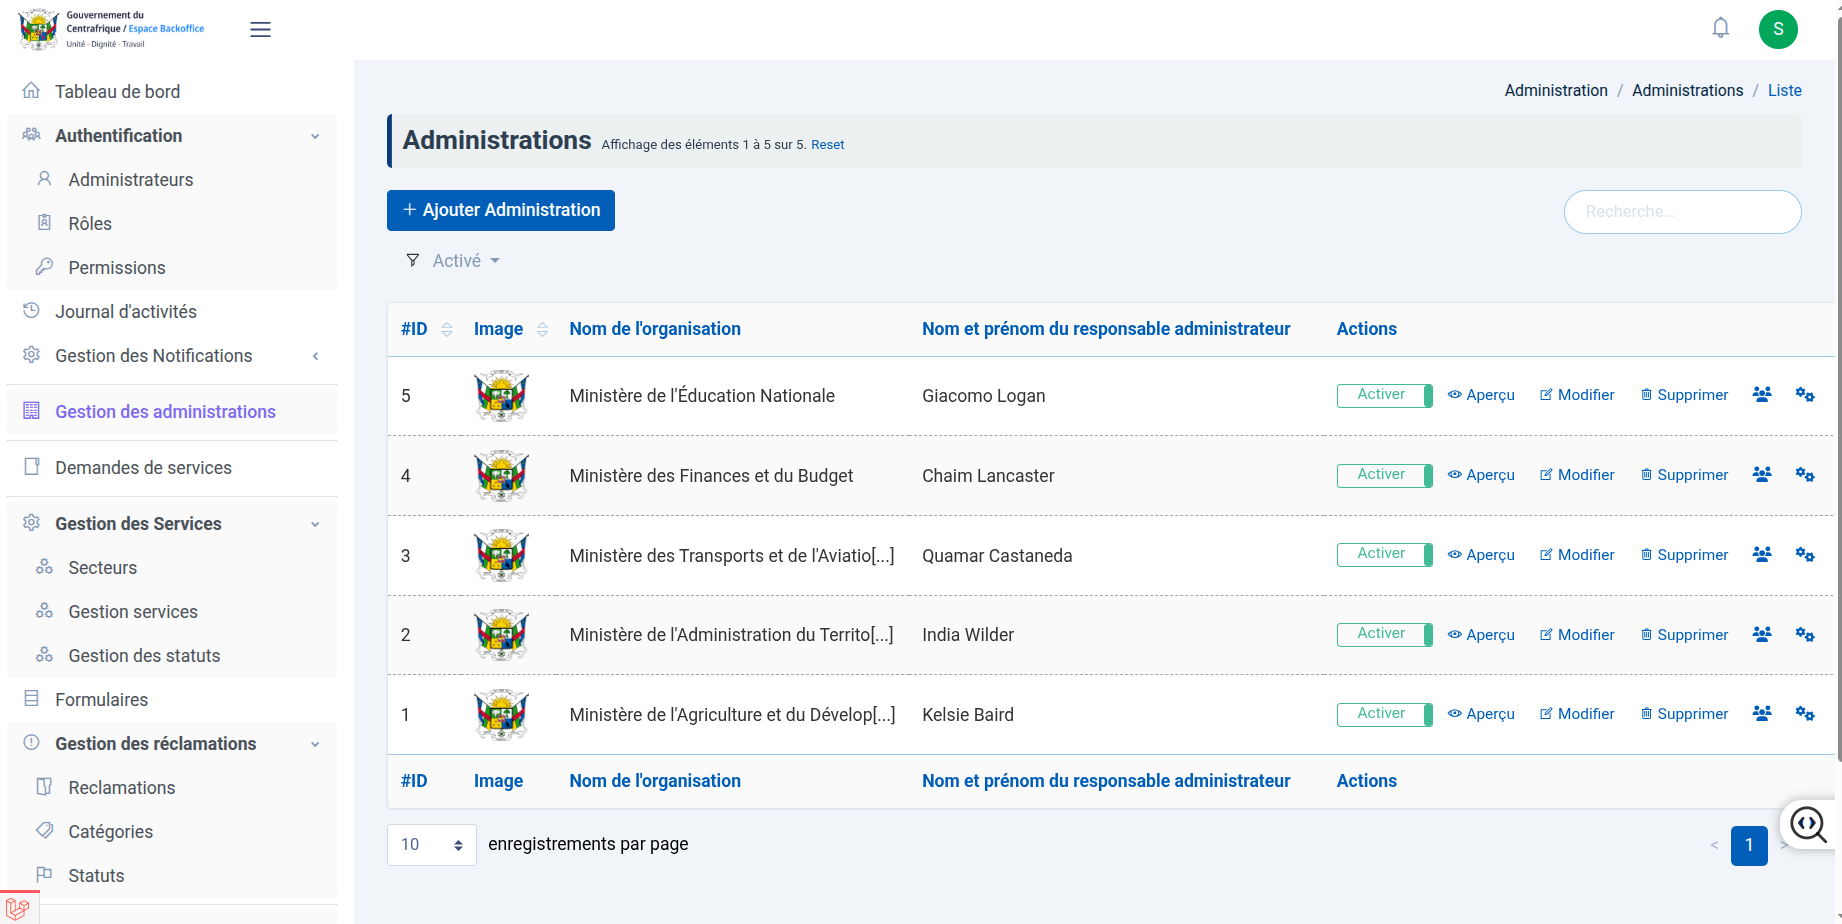
\includegraphics[width=0.95\textwidth]{images/realisation/sprint1/Capture1.png}
    }
    \caption{Liste des administrations}
    \label{fig:liste-admins}
\end{figure}

 

La figure~\ref{fig:liste-responsables} présente l’interface affichant la liste des responsables associés aux administrations offrant ainsi une vision claire de la structure organisationnelle et des rôles attribués au sein du système.






\begin{figure}[H]
    \centering
    \fbox{%
        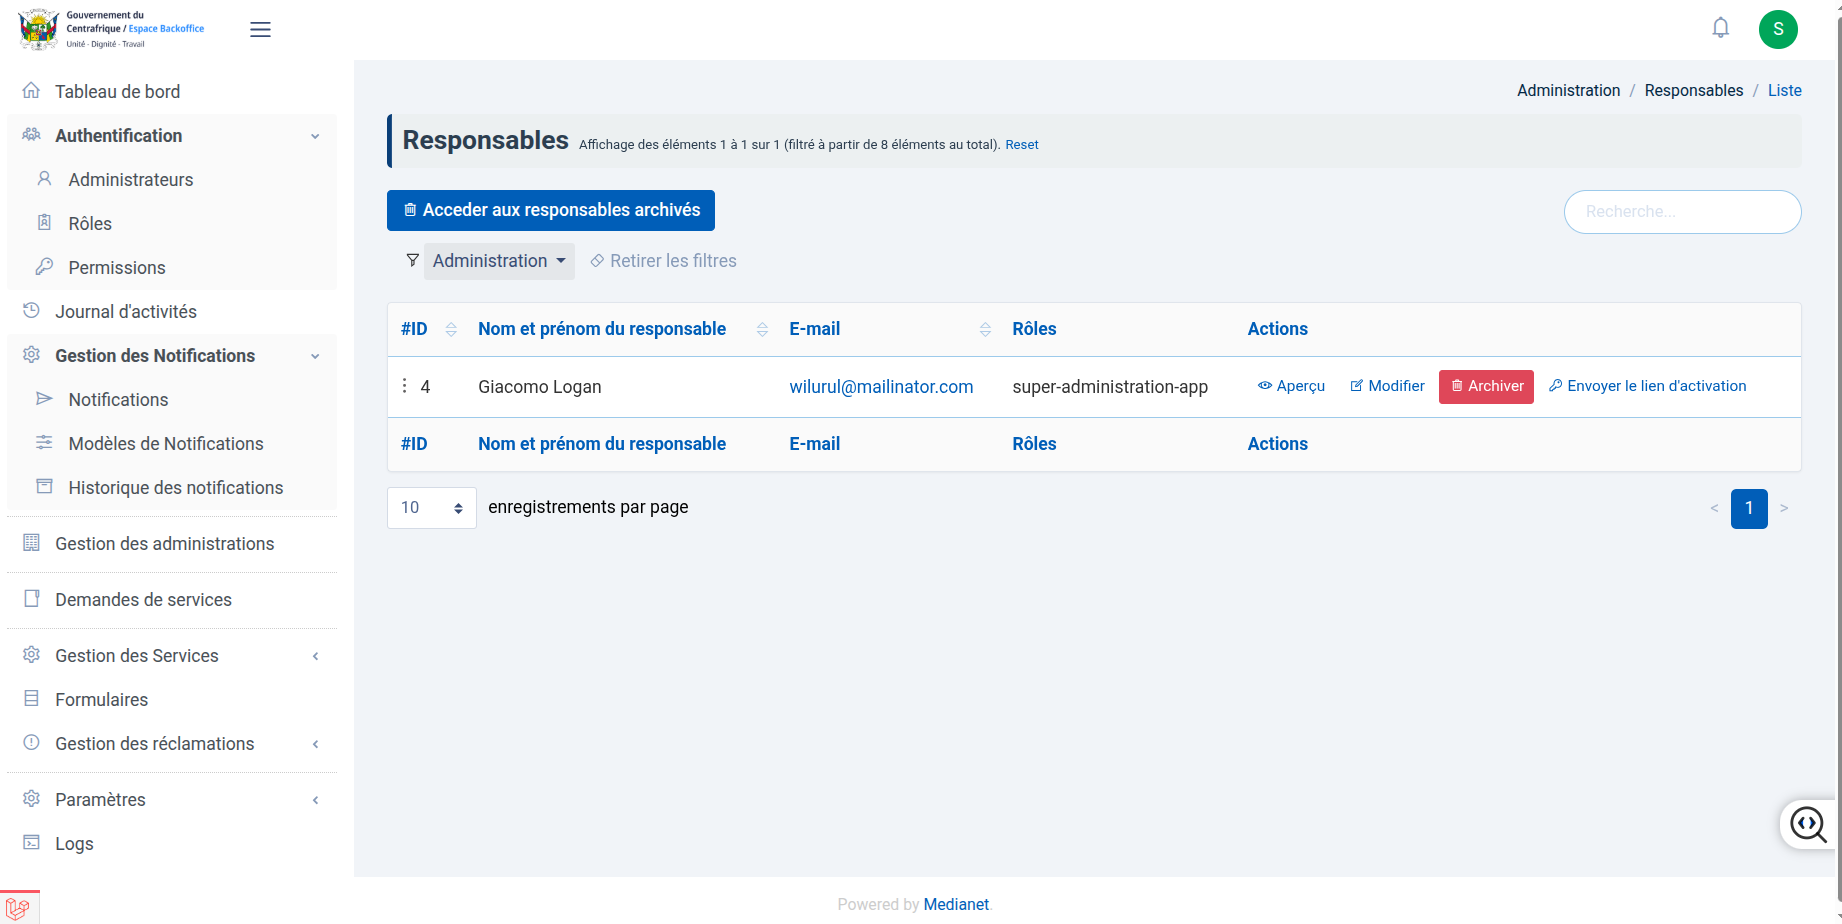
\includegraphics[width=0.95\textwidth]{images/realisation/sprint1/Capture2.png}
    }
       \caption{Liste des responsables de l’administration}
    \label{fig:liste-responsables}
\end{figure}
 

 

L’interface de création d’une nouvelle administration par l’administrateur où celui-ci doit saisir les informations requises notamment le nom les coordonnées et les données du responsable concerné est illustrée dans la figure~\ref{fig:ajouter-admin}.

\begin{figure}[H]
    \centering
    \fbox{%
        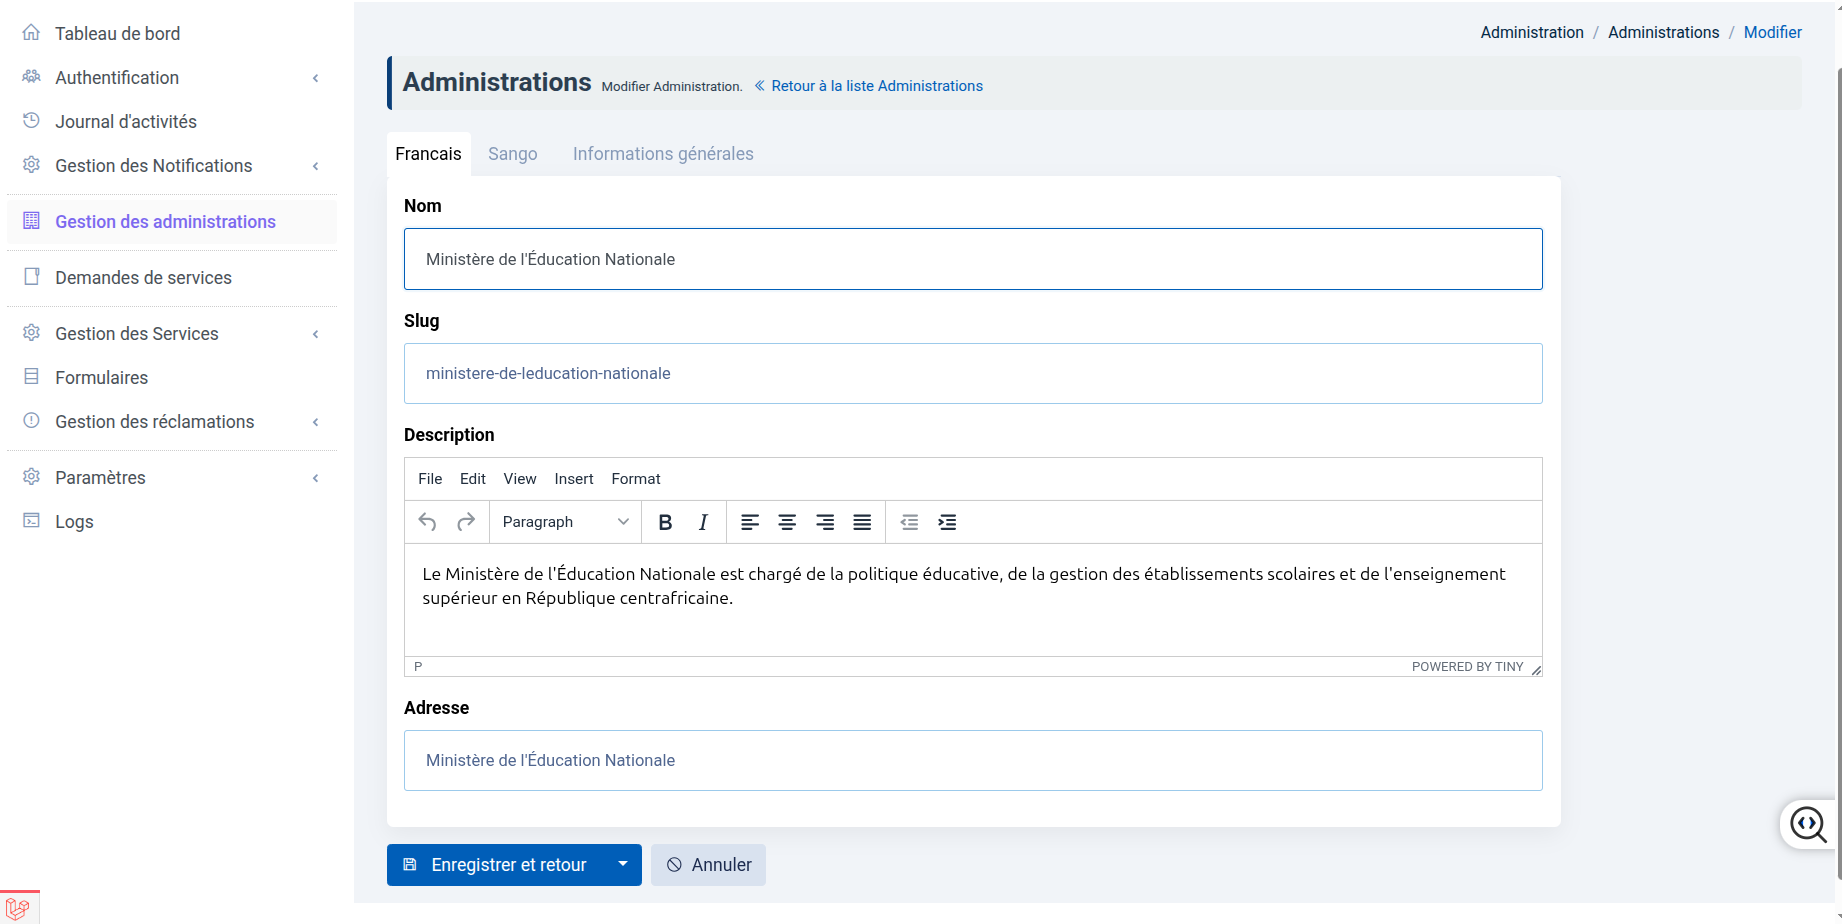
\includegraphics[width=0.95\textwidth]{images/realisation/sprint1/Capture3.png}
    }
    \caption{Ajouter une administration}
    \label{fig:ajouter-admin}
\end{figure}
 

La figure~\ref{fig:ajouter-responsable} présente l’interface permettant d’associer un administrateur institutionnel à une administration, en définissant ses informations, son rôle ainsi que ses permissions au sein de la structure administrative.

\begin{figure}[H]
    \centering
    \fbox{%
        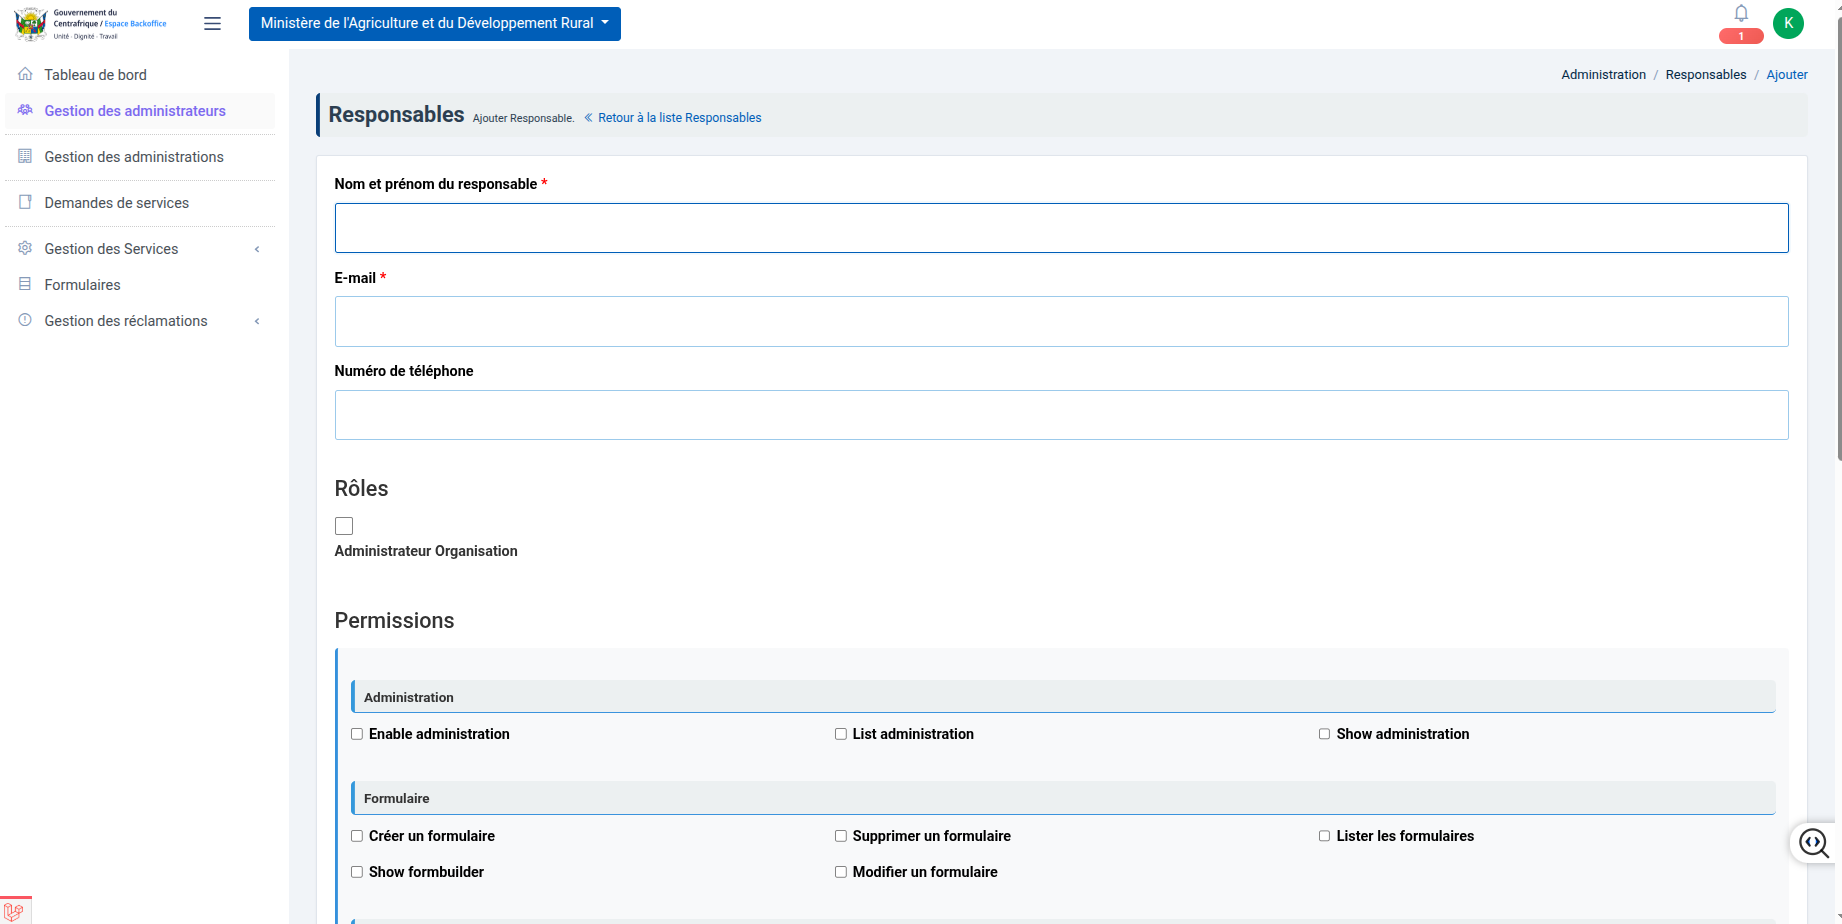
\includegraphics[width=0.95\textwidth]{images/realisation/sprint1/Capture4.png}
    }
    \caption{Ajouter un responsable à une administration}
    \label{fig:ajouter-responsable}
\end{figure}
















\subsection{Revue du Sprint 1}
À l’issue du Sprint 1, toutes les user stories prévues ont été développées et validées comme l’indique le tableau~\ref{tab:revue-sprint1}.

\begin{longtable}{|c|p{9cm}|c|}
\hline
\rowcolor{orange!30}
\textbf{ID} & \textbf{User Story} & \textbf{Statut} \\ \hline
US1 & S'authentifier & \textcolor{green!60!black}{Terminé} \\ \hline
US8 & Modifier mon profil & \textcolor{green!60!black}{Terminé} \\ \hline
US5 & Gérer les comptes des administrateurs institutionnels & \textcolor{green!60!black}{Terminé} \\ \hline
US7 & Gérer les langues de la plateforme & \textcolor{green!60!black}{Terminé} \\ \hline
US3 & Gérer les rôles & \textcolor{green!60!black}{Terminé} \\ \hline
US4 & Consulter les permissions & \textcolor{green!60!black}{Terminé} \\ \hline
US2 & Gérer les comptes des administrateurs backoffice & \textcolor{green!60!black}{Terminé} \\ \hline
US6 & Gérer les administrations ministérielles & \textcolor{green!60!black}{Terminé} \\ \hline
\caption{Revue du Sprint 1}
\label{tab:revue-sprint1}
\end{longtable}



\section{Sprint 2 : Catalogue de services et moteur de formulaires dynamiques}

Ce sprint établit le référentiel de services de la plateforme. Il donne aux administrateurs les outils nécessaires pour structurer l'offre de services par secteur, configurer des formulaires adaptés à chaque prestation et gérer les langues de l'interface. Il couvre également la partie citoyenne avec l'inscription, l'authentification et la consultation du catalogue de services.

\subsection{Backlog du Sprint 2}

Le tableau~\ref{tab:Backlogdu-sprint2} montre le backlog du sprint 2 avec l’estimation des tâches en jours.
 


\renewcommand{\arraystretch}{1.3}

\begin{longtable}{|p{1cm}|p{3cm}|p{7cm}|p{1cm}|p{2cm}|}

\hline
\rowcolor{orange!30}
\textbf{ID} & \textbf{En tant que} & \textbf{User Story} & \textbf{Est/J} & \textbf{Priorité} \\
\hline
\endfirsthead

 

US9  & Administrateur système &
Je veux gérer les secteurs de services afin d'organiser les offres de la plateforme par domaine &
2 & Élevée \\ \hline

US10 & Administrateur ministériel &
Je veux gérer les services administratifs afin de définir les prestations disponibles pour les citoyens &
4 & Élevée \\ \hline

US11 & Administrateur institutionnel &
Je veux gérer le moteur de formulaires dynamiques afin de personnaliser les champs et les étapes des demandes par service &
8 & Élevée \\ \hline

US12 & Internaute &
Je veux créer un compte afin de pouvoir déposer des demandes de services &
2 & Élevée \\ \hline

US13 & Client &
Je veux m'authentifier afin d'accéder à mon espace personnel &
2 & Élevée \\ \hline

US14 & Internaute &
Je veux consulter les secteurs et les services disponibles afin de connaître les offres par administration &
2 & Moyenne \\ \hline

\caption{Backlog du Sprint 2}
\label{tab:Backlogdu-sprint2}

\end{longtable}

 

\subsection{Diagramme de cas d'utilisation du sprint 2}
Le diagramme de cas d'utilisation du sprint 2 est représenté par la figure \ref{fig:cas-utilisation-sprint2}.

\begin{figure}[H]
    \centering
    \includegraphics[width=10cm,height=15cm]{images/diagrammes/sprint2/diag-utili-speint2.drawio.png}
    \caption{Diagramme de cas d'utilisation -- Sprint 2}
    \label{fig:cas-utilisation-sprint2}
\end{figure}

\subsection{Diagramme de classe du sprint 2}
Le diagramme de classe du sprint 2 est présenté dans la figure \ref{fig:Diagrammedeclasse-Sprint2}.

\begin{figure}[H]
    \centering
    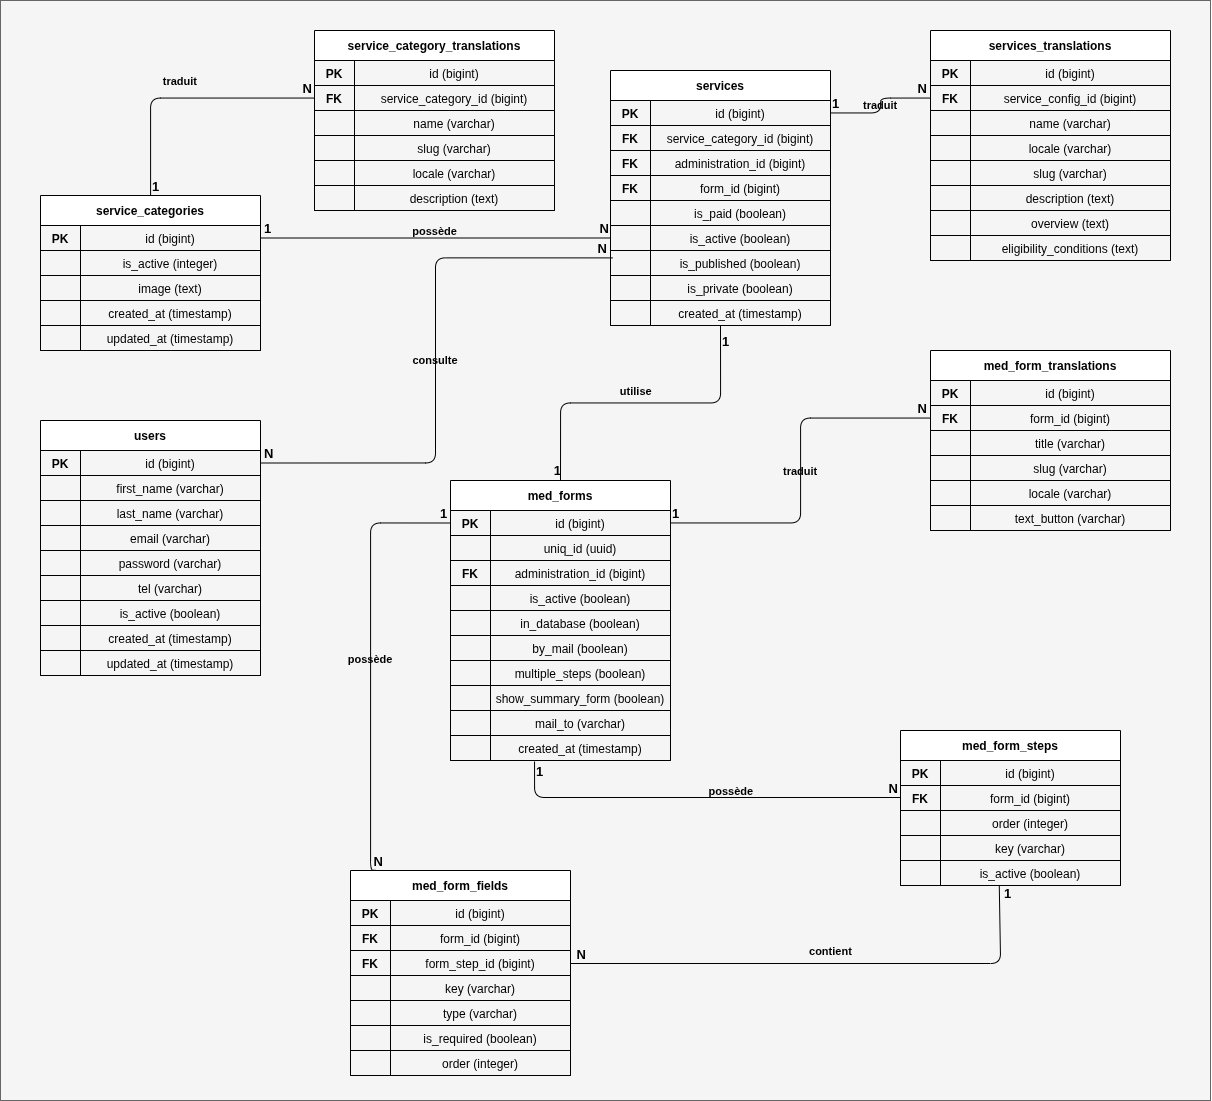
\includegraphics[width=16cm,height=15cm]{images/diagrammes/sprint2/diag-classe-sprint2.drawio.png}
    \caption{Diagramme de classe -- Sprint 2}
    \label{fig:Diagrammedeclasse-Sprint2}
\end{figure}


\subsection{Raffinement et description textuelle du cas d'utilisation <<Gérer les formulaires dynamiques >>}

Dans cette section , nous utiliserons des descriptions de
scénarios pour décrire le cas « Gérer les formulaires dynamiques ». Ce dernier montre les sous-opérations possibles à faire.


La figure \ref{fig:cas-utilisation-sprint2-raff} montre le diagramme de cas d'utilisation affiné du cas d'utilisation « Gérer les formulaires dynamiques ».

\begin{figure}[H]
    \centering
    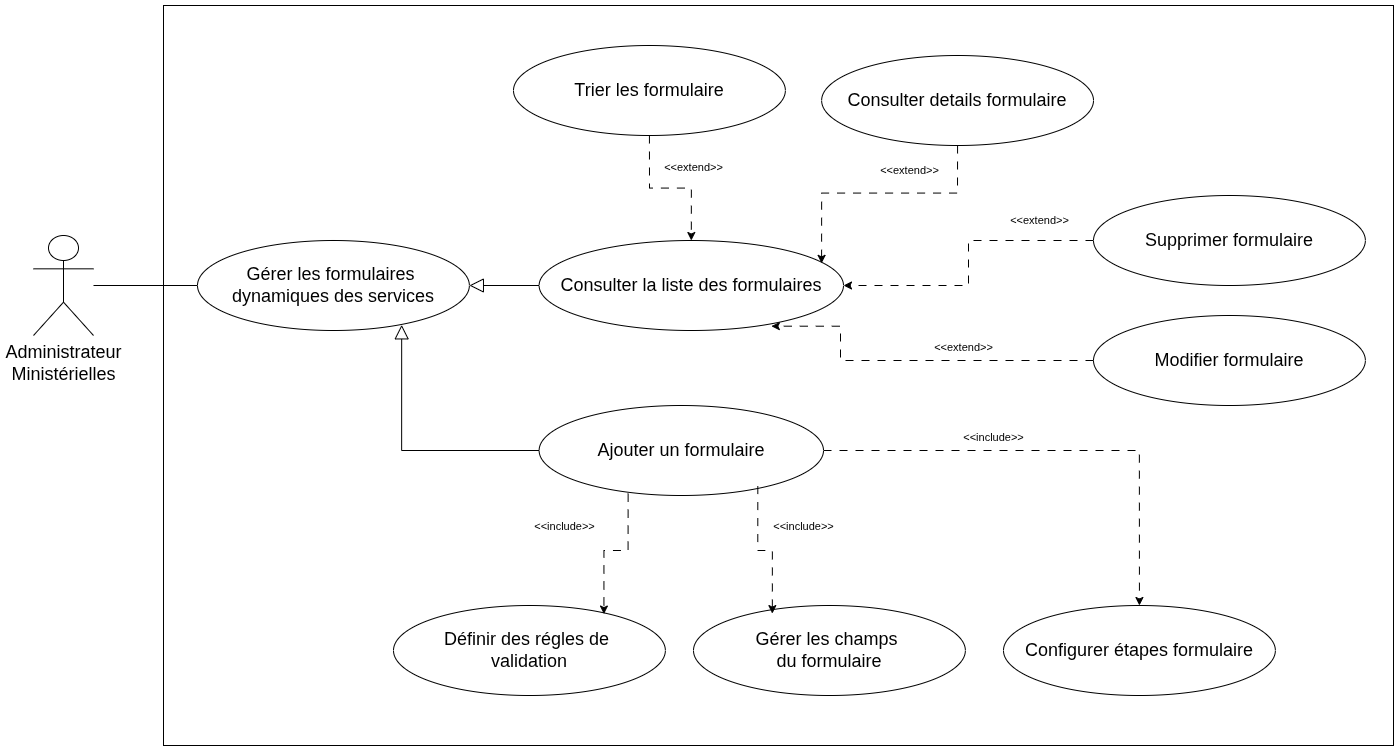
\includegraphics[width=15cm,height=8cm]{images/diagrammes/sprint2/cas-utilisation-form-dyn.drawio.png}
    \caption{Raffinement du cas d'utilisation « Gérer les formulaires dynamiques »}
    \label{fig:cas-utilisation-sprint2-raff}
\end{figure}

\textbf{Description textuelle}


Une description détaillée du cas d’utilisation « Consulter un formulaire dynamique » est présentée ci-dessous dans le tableau~\ref{tab:uc-preview}.


 
\begin{longtable}{|p{4cm}|p{12cm}|}
\hline

\rowcolor{gray!20}
\textbf{Champ} & \textbf{Description} \\ \hline
\endfirsthead

 

Nom & Consulter détails formulaire \\ \hline

Acteur principal & Administrateur \\ \hline

Objectif & Vérifier le rendu et le comportement du formulaire avant sa publication. \\ \hline

Pré-condition &
\begin{itemize}
    \item Le formulaire est créé.
\end{itemize}
\\ \hline

Scénario nominal &
\begin{enumerate}
    \item L’administrateur clique sur "Aperçu".
    \item Le système affiche le formulaire.
    \item L’administrateur vérifie le rendu.
\end{enumerate}
\\ \hline

Scénario alternatif &
\begin{itemize}
    \item En cas d’erreur de chargement, le système affiche un message d’erreur.
\end{itemize}
\\ \hline

Post-condition & Le formulaire est validé ou corrigé avant publication. \\ \hline

\caption{Description textuelle : Consulter détails formulaire}
\label{tab:uc-preview}

\end{longtable}
 


Une description détaillée du cas d’utilisation « Modifier un formulaire dynamique » est présentée ci-dessous dans le tableau~\ref{tab:uc-edit-formulaire-dynamique}.


\begin{longtable}{|p{3cm}|p{13cm}|}
\hline

\rowcolor{gray!20}
\textbf{Champ} & \textbf{Description} \\ \hline
\endfirsthead

 

Nom & Modifier un formulaire dynamique \\ \hline

Acteur principal & Administrateur \\ \hline

Objectif & Permettre à l’administrateur de mettre à jour et de reconfigurer un formulaire dynamique existant afin de l’adapter aux besoins changeants. \\ \hline

Pré-condition &
\begin{itemize}
    \item L’administrateur est authentifié.
    \item L’administrateur dispose des droits nécessaires.
    \item Le formulaire dynamique existe dans le système.
\end{itemize}
\\ \hline

Scénario nominal &
\begin{enumerate}
    \item L'administrateur accède au module de gestion des formulaires.
    \item Il vérifie la liste des formulaires existants.
    \item Il choisit un formulaire dynamique à modifier.
    \item Le système présente les données du formulaire (nom, description, service associé, champs, steps et validations).
    \item L'administrateur modifie les données générales du formulaire.
    \item Il ajoute, modifie ou supprime des champs (texte, date, fichier, liste déroulante, ...).
    \item Il modifie les règles de validation des champs ainsi que leurs propriétés.
    \item Il réorganise les champs dans les différents pas (steps) du formulaire.
    \item Le système vérifie que la structure du formulaire est cohérente.
    \item L'administrateur vérifie les modifications.
    \item Le système enregistre les modifications apportées.
    \item Le système présente un message de confirmation.
\end{enumerate}
\\ \hline

Scénario alternatif &
\begin{itemize}
    \item Si un champ comporte une configuration non valide, le système génère un message d’erreur et empêche l’enregistrement.
    \item Si une étape est vide, le système bloque son enregistrement.
    \item Si l'opération est annulée par l'administrateur, aucune modification n'est enregistrée.
    \item Si le formulaire n'existe plus, le système affiche une erreur.
\end{itemize}
\\ \hline

Post-condition & Le formulaire dynamique est mis à jour avec sa nouvelle structure. \\ \hline

\caption{Description textuelle du cas d'utilisation : Modifier un formulaire dynamique}
\label{tab:uc-edit-formulaire-dynamique}

\end{longtable}


\subsection{Les diagrammes de séquences du cas d’utilisation « Gérer les formulaires dynamiques »}

Dans cette partie, nous avons choisi de ne présenter que quelques-uns des diagrammes de séquence identifiés lors du pas de raffinement. Ce choix permet de mettre en évidence les interactions les plus représentatives du cas d’utilisation « Gérer les formulaires dynamiques », notamment les opérations essentielles la modification et la consultation. Ces diagrammes permettent d’illustrer plus clairement le fonctionnement du système ainsi que les échanges entre les différents acteurs et les composants applicatifs.

\noindent  \textbf{Présentation des diagrammes de séquences :}

% Modifier
Le diagramme de la figure~\ref{fig:modif-form} montre le processus de modification d’un formulaire dynamique, qui permet à l’administrateur d’éditer les champs, les étapes et les règles de validation avant la mise à jour des données dans le système.  

\begin{figure}[H]
    \centering
    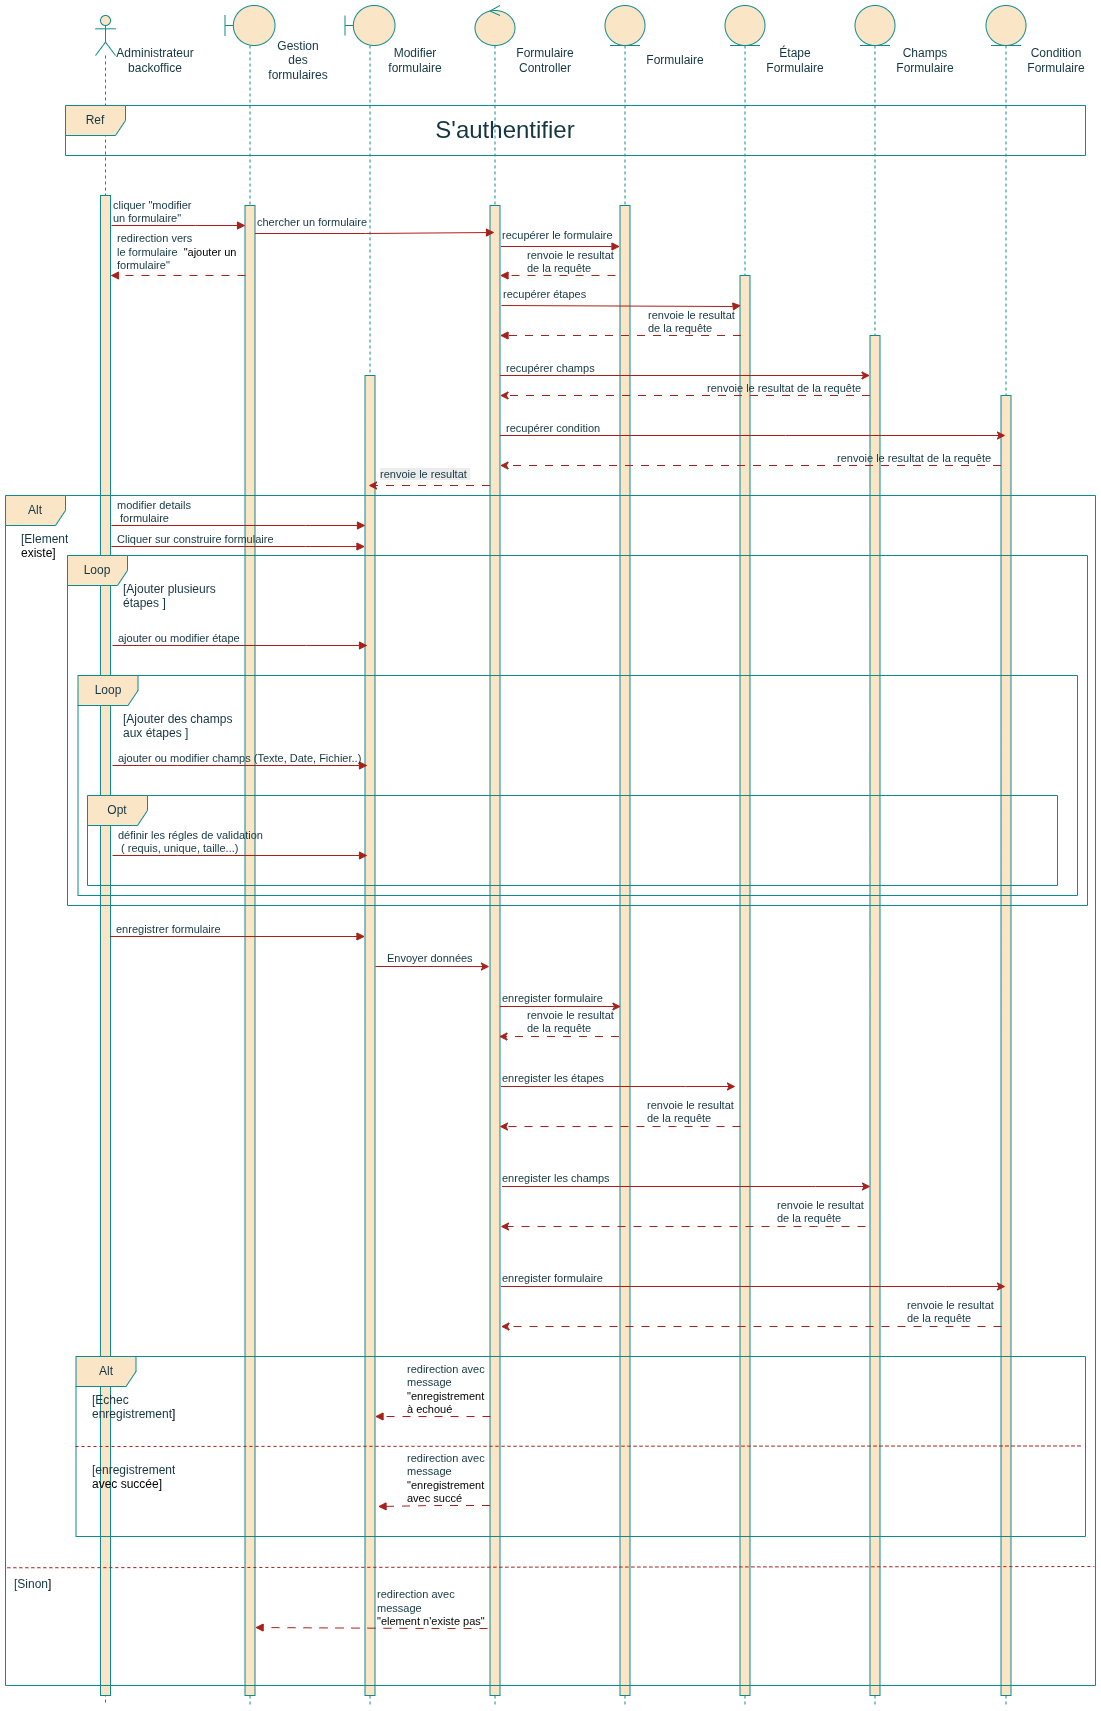
\includegraphics[width=18cm,height=23cm]{images/diagrammes/sprint2/modif-formulaire.drawio.png}
    \caption{Diagramme de séquence - Modifier un formulaire}
    \label{fig:modif-form}
\end{figure}

 
% Consulter
Le diagramme présenté à la figure~\ref{fig:consulter-form}, décrit le processus de consultation des formulaires dynamiques et permet à l’administrateur de visualiser la liste des formulaires ainsi que leurs détails et configurations.

\begin{figure}[H]
    \centering
    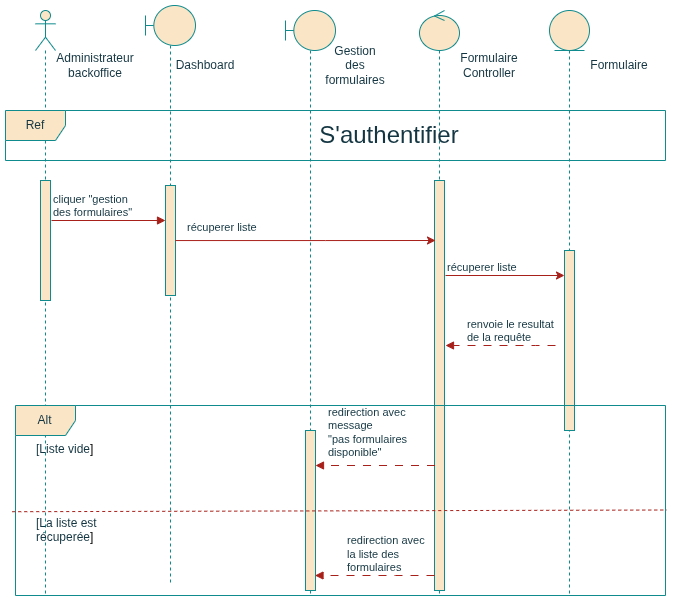
\includegraphics[width=18cm,height=16cm]{images/diagrammes/sprint2/consulter-formulai.drawio.png}
    \caption{Diagramme de séquence - Consulter un formulaire}
    \label{fig:consulter-form}
\end{figure}

\subsection{Réalisation du sprint « Gérer formulaire dynamique »}

Dans cette section nous avons choisi de présenter certaines interfaces représentatives du sprint « Gérer formulaire dynamique » afin d’illustrer les principales fonctionnalités implémentées. Ce choix met en avant les écrans les plus significatifs du système, notamment la consultation, l’ajout, la configuration et la modification des formulaires. Ces captures permettent de mieux appréhender le fonctionnement global de l’application ainsi que l’interaction de l’administrateur avec les différentes fonctionnalités proposées.


\noindent \textbf{Présentation des interfaces :}

La figure~\ref{fig:real1} présente l'interface de l'administrateur qui permet de consulter tous les formulaires enregistrés dans le système. Cette interface permet également de rechercher, de filtrer et d’accéder aux opérations de gestion associées.






\begin{figure}[H]
    \centering
    \fbox{%
        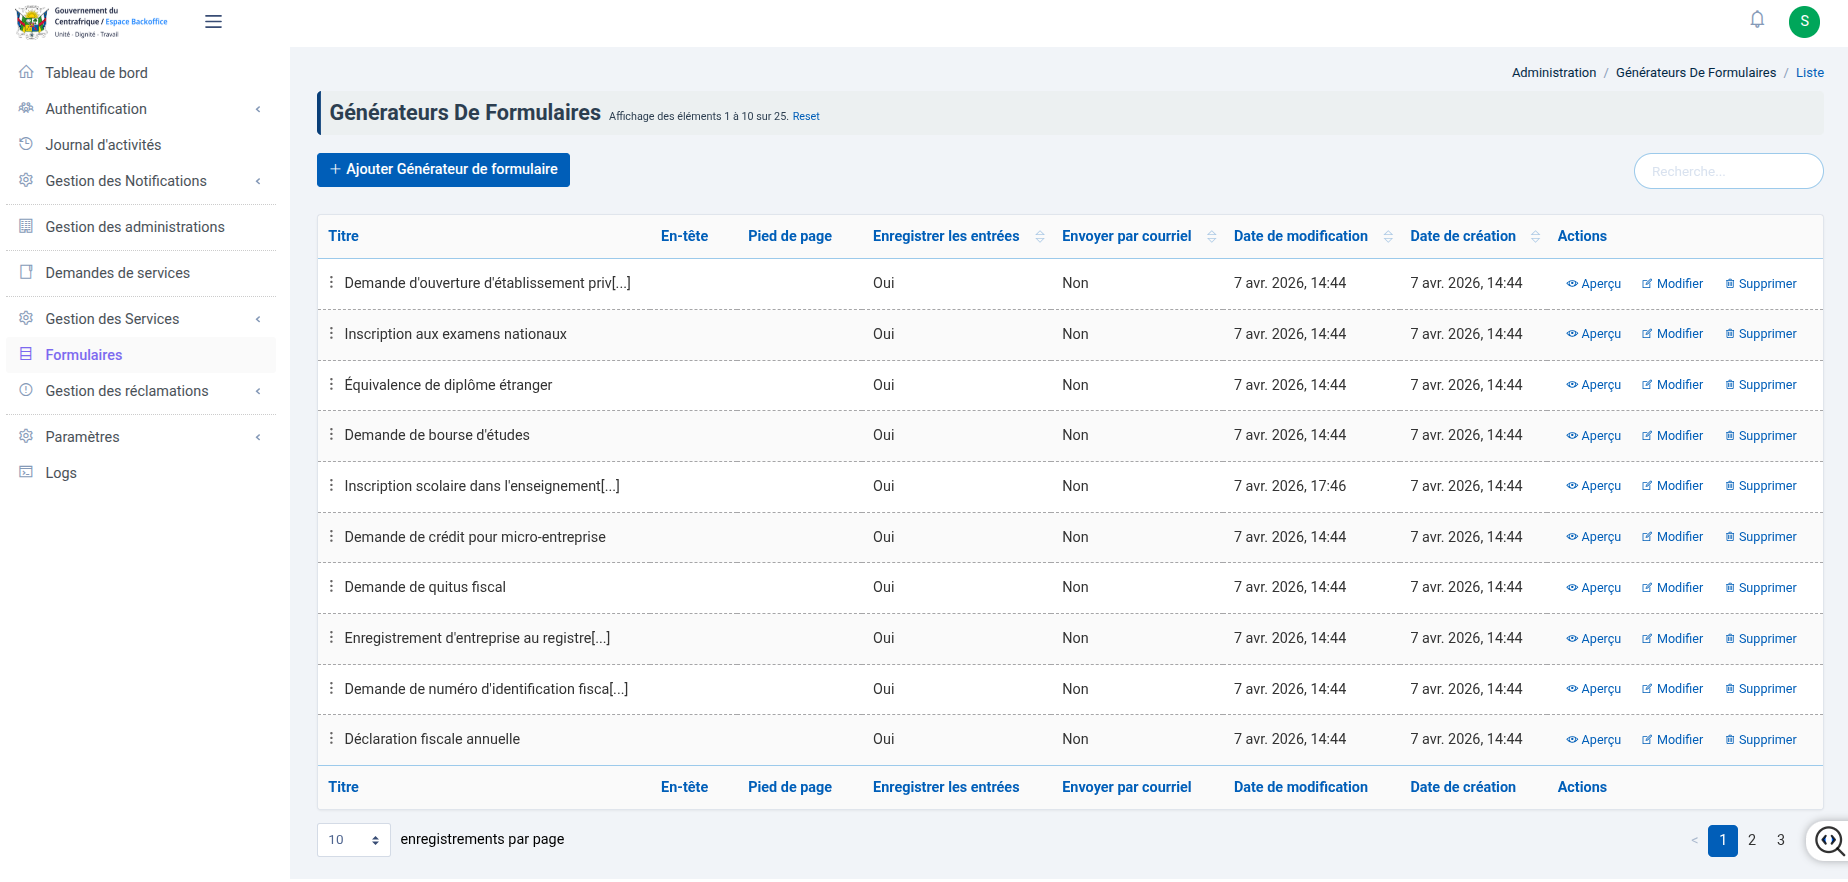
\includegraphics[width=0.95\textwidth]{images/realisation/sprint2/consulter-sprint2.png}
    }
    \caption{Liste des formulaires}
    \label{fig:real1}
\end{figure}

La figure~\ref{fig:real2} montre l'interface qui permet à l’administrateur d'ajouter de nouveaux formulaires dynamiques dans le système.



\begin{figure}[H]
    \centering
    \fbox{%
        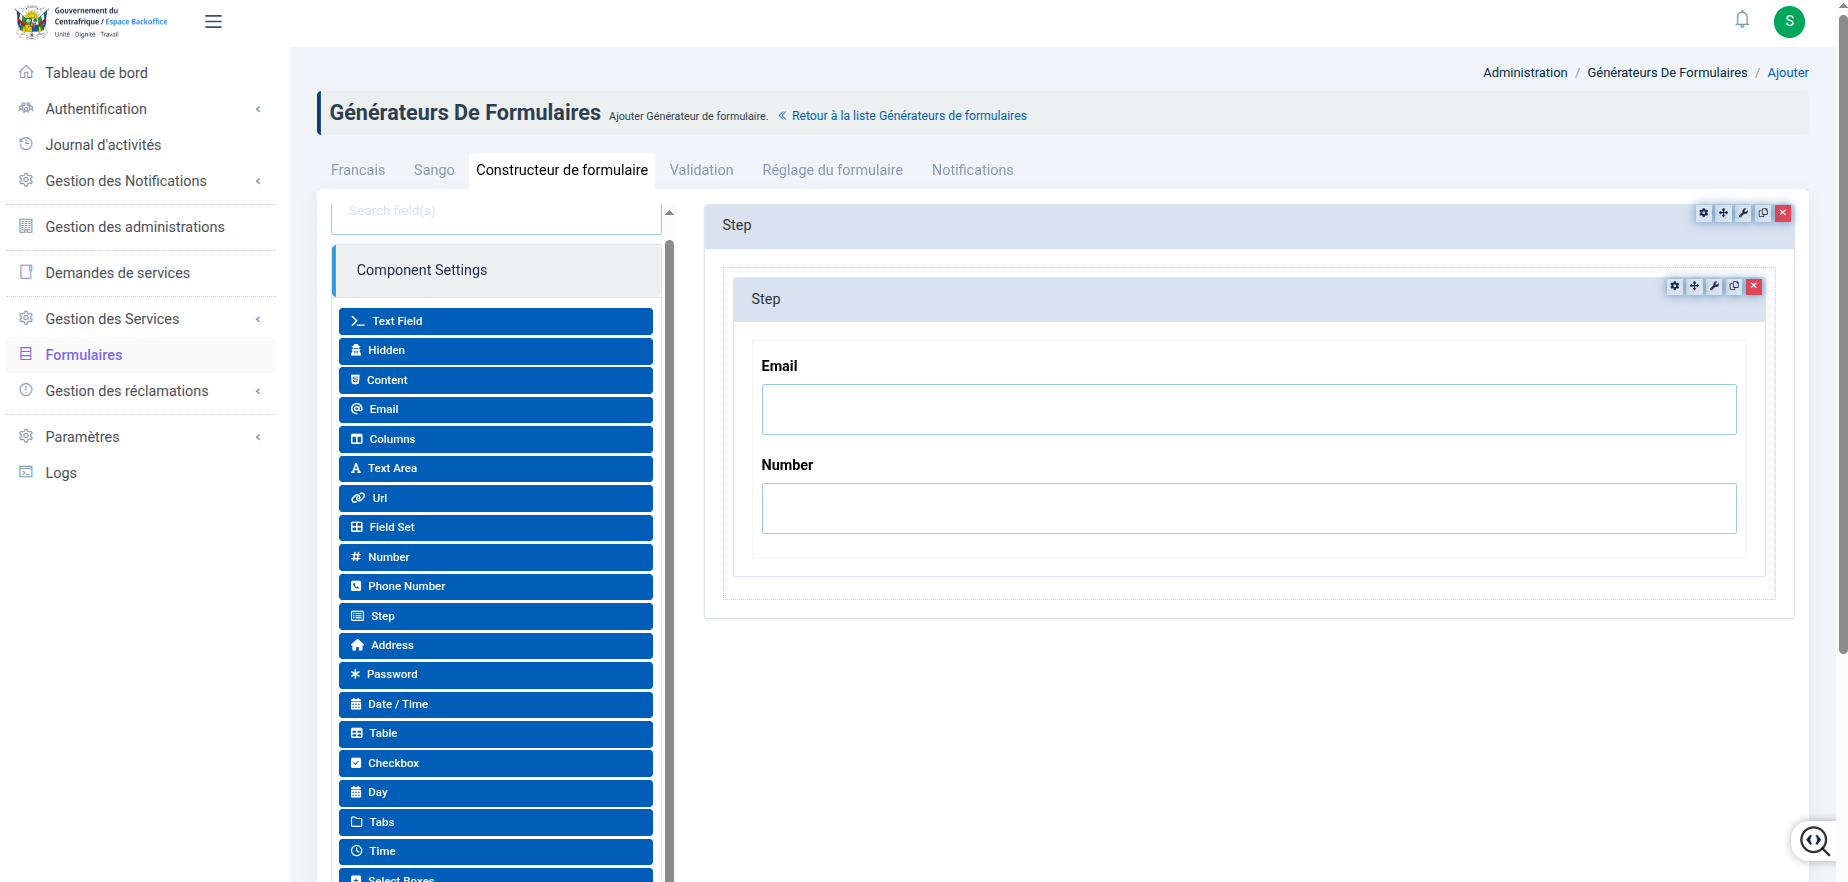
\includegraphics[width=0.95\textwidth]{images/realisation/sprint2/add-list.png}
    }
    \caption{Ajout des formulaires}
    \label{fig:real2}
\end{figure}






La figure~\ref{fig:real3} présente l'interface qui permet à l’administrateur de configurer les différents paramètres d'un champ, par exemple le champ CIN dans le cas suivant.
 





\begin{figure}[H]
    \centering
    \fbox{%
        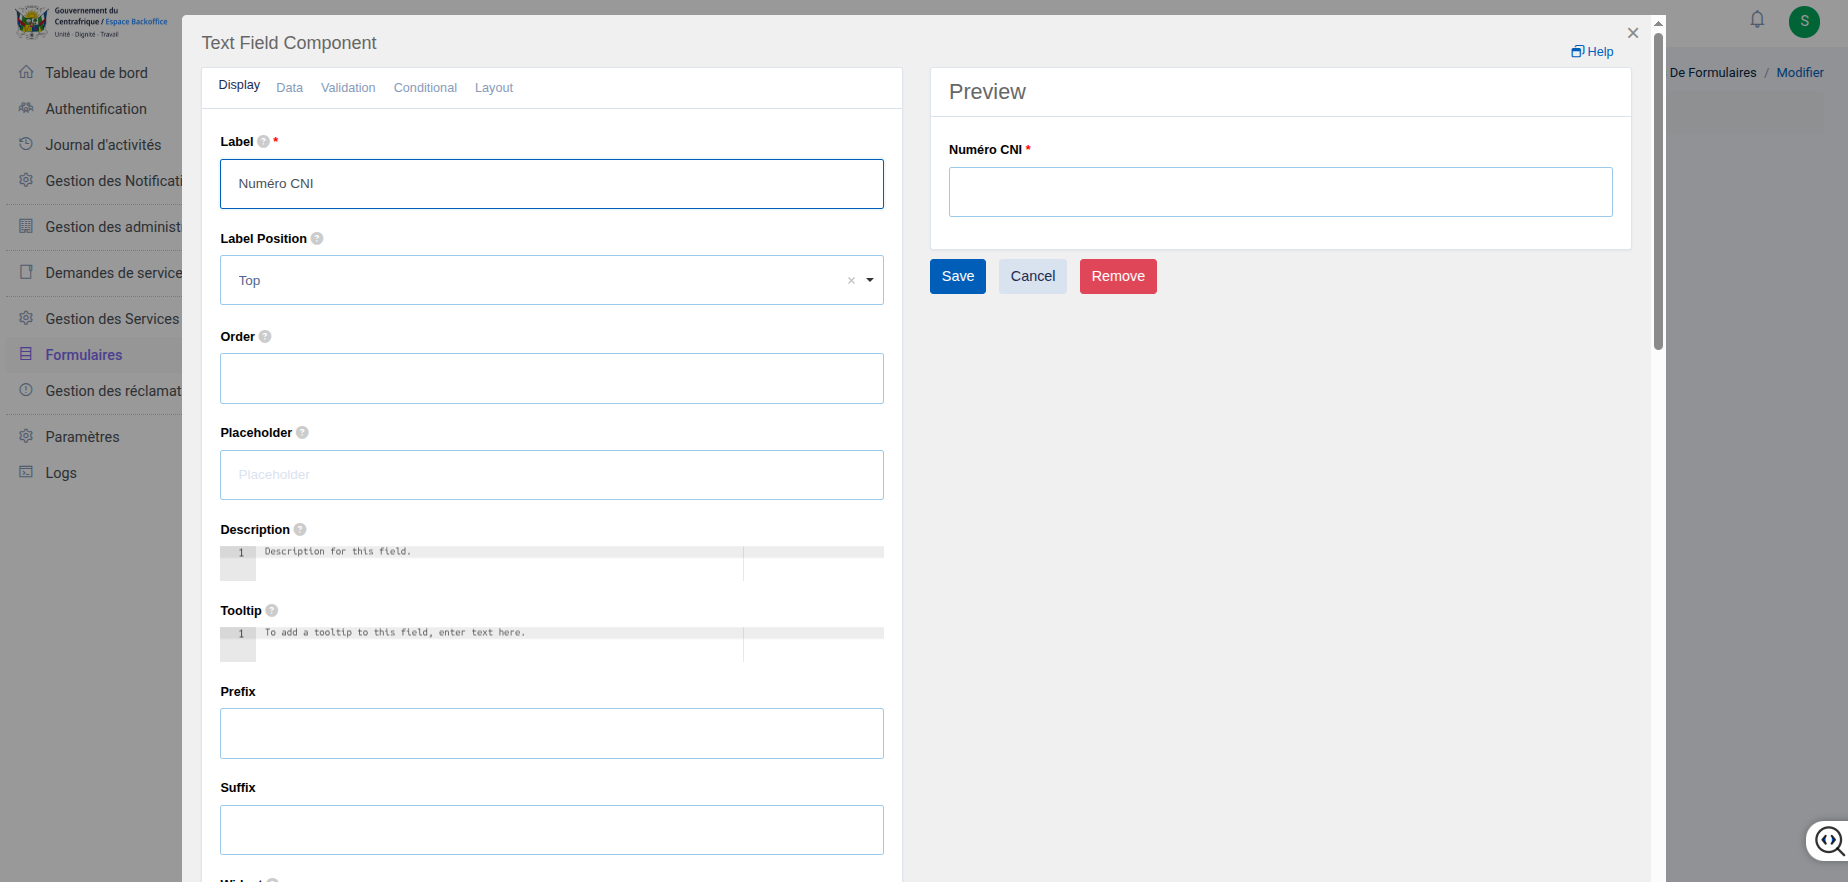
\includegraphics[width=0.95\textwidth]{images/realisation/sprint2/Capture d’écran du 2026-04-16 12-03-09.png}
    }
    \caption{Configuration des champs du formulaire}
    \label{fig:real3}
\end{figure}

La figure~\ref{fig:real4} présente l'interface qui permet à l’administrateur de modifier un formulaire existant en mettant à jour ses champs, ses étapes et ses règles de validation.

 

\begin{figure}[H]
    \centering
    \fbox{%
        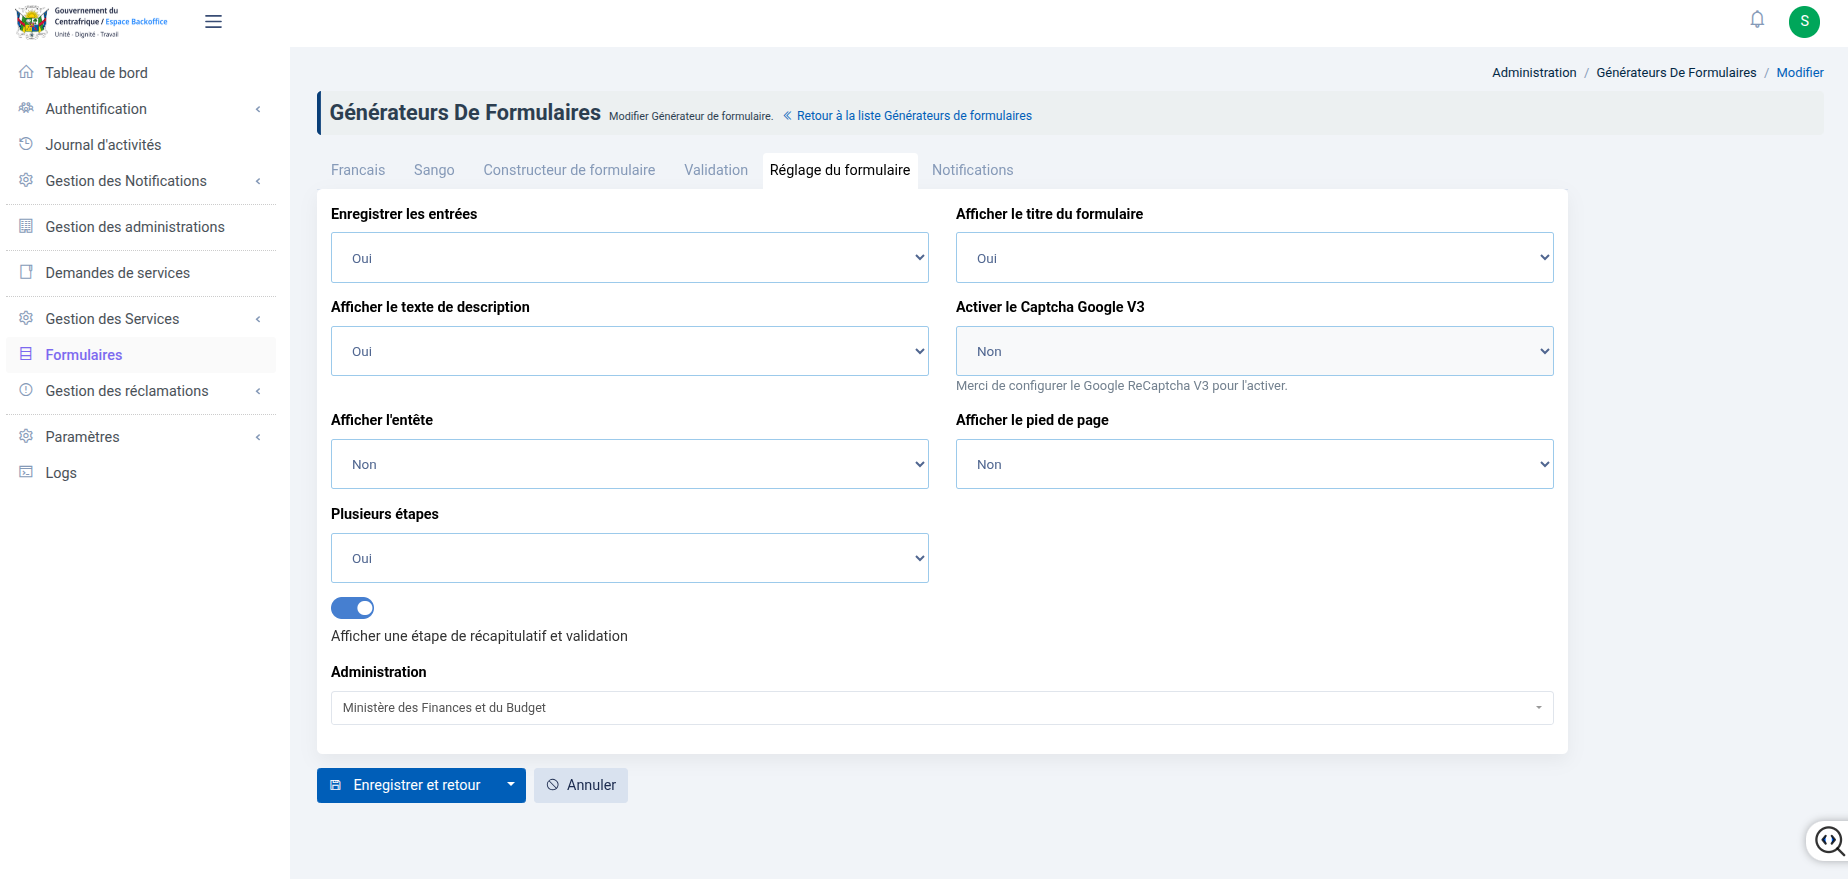
\includegraphics[width=0.95\textwidth]{images/realisation/sprint2/Capture d’écran du 2026-04-16 12-05-36.png}
    }
    \caption{Modification d’un formulaire}
    \label{fig:real4}
\end{figure}
 
\subsection{Revue du Sprint 2}
 

A l'issue du Sprint 2 l'ensemble des user stories planifiées ont été développées et validées comme présenté dans le tableau~\ref{tab:revue-sprint2}.

\newpage

\begin{longtable}{|c|p{9cm}|c|}
\hline
\rowcolor{orange!30}
\textbf{ID} & \textbf{User Story} & \textbf{Statut} \\ \hline
US9  & Gérer les secteurs de services & \textcolor{green!60!black}{Terminé} \\ \hline
US10 & Gérer les services administratifs & \textcolor{green!60!black}{Terminé} \\ \hline
US12 & Gérer le moteur de formulaires dynamiques & \textcolor{green!60!black}{Terminé} \\ \hline
US13 & Créer un compte citoyen & \textcolor{green!60!black}{Terminé} \\ \hline
US14 & S’authentifier (Client) & \textcolor{green!60!black}{Terminé} \\ \hline
US15 & Consulter les secteurs et les services disponibles & \textcolor{green!60!black}{Terminé} \\ \hline
\caption{Revue du Sprint 2}
\label{tab:revue-sprint2}
\end{longtable}

\section{Sprint 3 : Dématérialisation et suivi des démarches en ligne}

Le Sprint 3 constitue une étape clé du projet, dédiée à la dématérialisation des demandes de services. Il permet aux citoyens de soumettre et suivre leurs dossiers, de fournir des informations complémentaires et d’évaluer les services, tout en offrant un tableau de bord personnalisé.

Du côté des administrations, il introduit la gestion et le suivi des demandes ainsi que la personnalisation des étapes de traitement selon les besoins spécifiques.

Enfin, ce sprint intègre également des fonctionnalités complémentaires telles que la modification du profil utilisateur afin d’améliorer l’expérience globale.


\subsection{Backlog du Sprint 3}

Le tableau ci-dessous présente le backlog du troisième sprint avec l'estimation en jours de chaque tâche.

\begin{table}[H]
    \centering
    \begin{tabular}{ |p{1cm}|p{3cm}|p{7cm}|p{1cm}|p{2cm}|} \hline
    \rowcolor{orange!30}
    \textbf{ID} & \textbf{En tant que} & \textbf{User Story} & \textbf{Est/J} & \textbf{Priorité} \\ \hline
    
    US15 & Administrateur Ministériel & Je veux personnaliser les étapes de traitement des demandes sur les services afin d’adapter le workflow aux besoins spécifiques de mon ministère & 2 & Élevée \\ \hline

    US16 & Client & Je veux déposer une demande de service en ligne afin d'obtenir une prestation administrative sans me déplacer & 7 & Élevée \\ \hline

    US17 & Client & Je veux suivre l'état d'avancement de mes dossiers afin de connaître leur progression en temps réel & 4 & Élevée \\ \hline

    US18 & Client & Je veux évaluer un service après traitement afin de donner mon avis sur la qualité de la prestation & 2 & Moyenne \\ \hline

    US19 & Client & Je veux consulter mon tableau de bord afin d’avoir une vue d’ensemble de mes demandes et activités & 2 & Moyenne \\ \hline

    US20 & Client & Je veux Modifier mon profil afin de changer mes informations personnelles & 1 & Moyenne \\ \hline

    US21 & Administrateur Institutionnel & Je veux gérer les demandes de service afin de les traiter et les suivre & 2 & Élevée \\ \hline

    \end{tabular}
    \caption{User stories du Sprint 3}
    \label{tab:user-stories-sprint3}
\end{table}

\subsection{Spécification fonctionnelle du Sprint 3}

Dans cette section nous présentons les diagrammes de cas d'utilisation du sprint 3 le raffinement des cas principaux ainsi que leur description textuelle.

\subsection{Diagramme de cas d'utilisation du sprint 3}
La figure \ref{fig:cas-utilisation-sprint3}, présente le diagramme de cas d'utilisation du sprint 3.

\begin{figure}[H]
    \centering
    \includegraphics[width=12cm,height=14cm]{images/diagrammes/sprint3/diag-classe-sprint3.drawio.png}
    \caption{Diagramme de cas d'utilisation -- Sprint 3}
    \label{fig:cas-utilisation-sprint3}
\end{figure}

\subsection{Diagramme de classe du sprint 3}
La figure \ref{fig:class-sprint3} présente le diagramme de classe du sprint 3.
\begin{figure}[H]
    \centering
    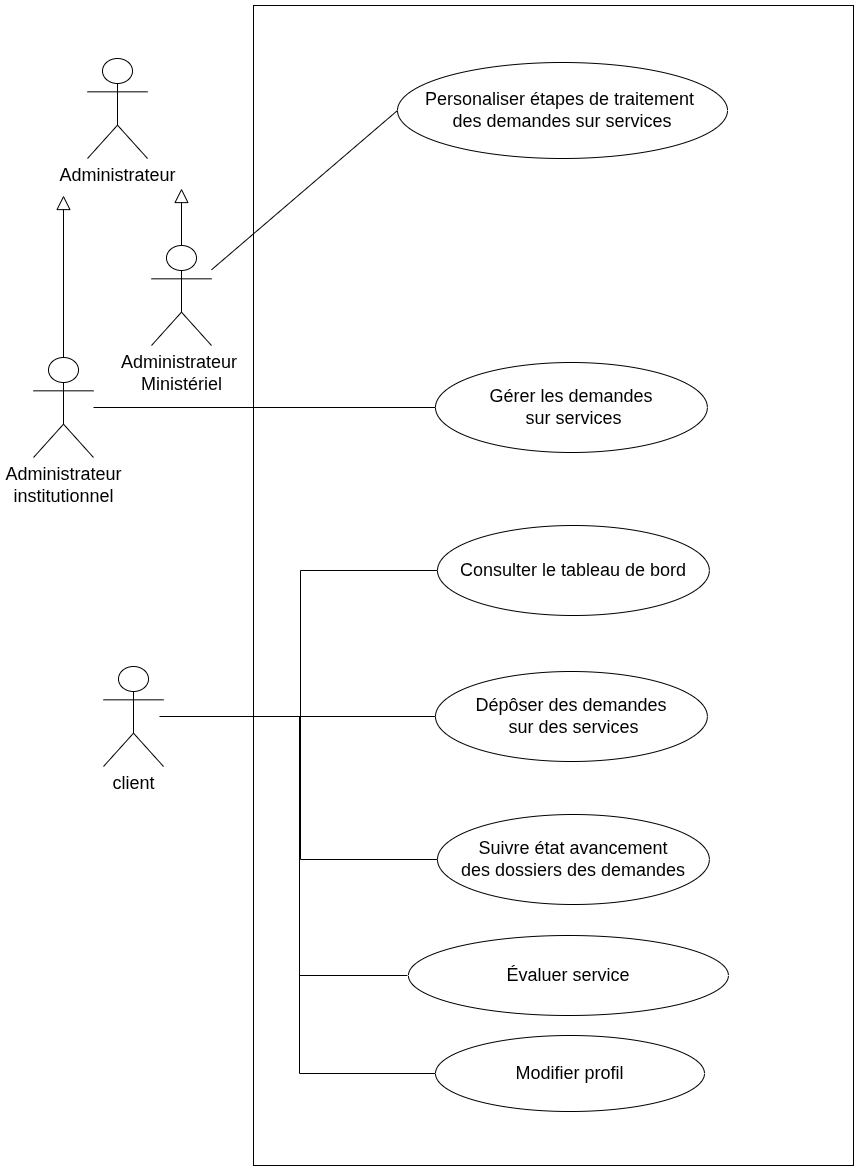
\includegraphics[width=16cm,height=16cm]{images/diagrammes/sprint3/cas-utilisation-sprint3.drawio.png}
    \caption{Diagramme de classe -- Sprint 3}
    \label{fig:class-sprint3}
\end{figure}

\subsection{Raffinement et description textuelle du cas d'utilisation << Suivre état avancement des dossiers des demandes >>}

Dans la section suivante, nous utiliserons des descriptions de
scénarios pour décrire le cas « Suivre état avancement des dossiers des demandes ». Ce dernier montre les sous-opérations possibles à faire.

La figure \ref{fig:cas-utilisation-sprint3-raff} montre le diagramme de cas d'utilisation raffiné du cas d'utilisation « Suivre état avancement des dossiers des demandes ».

\begin{figure}[H]
    \centering
    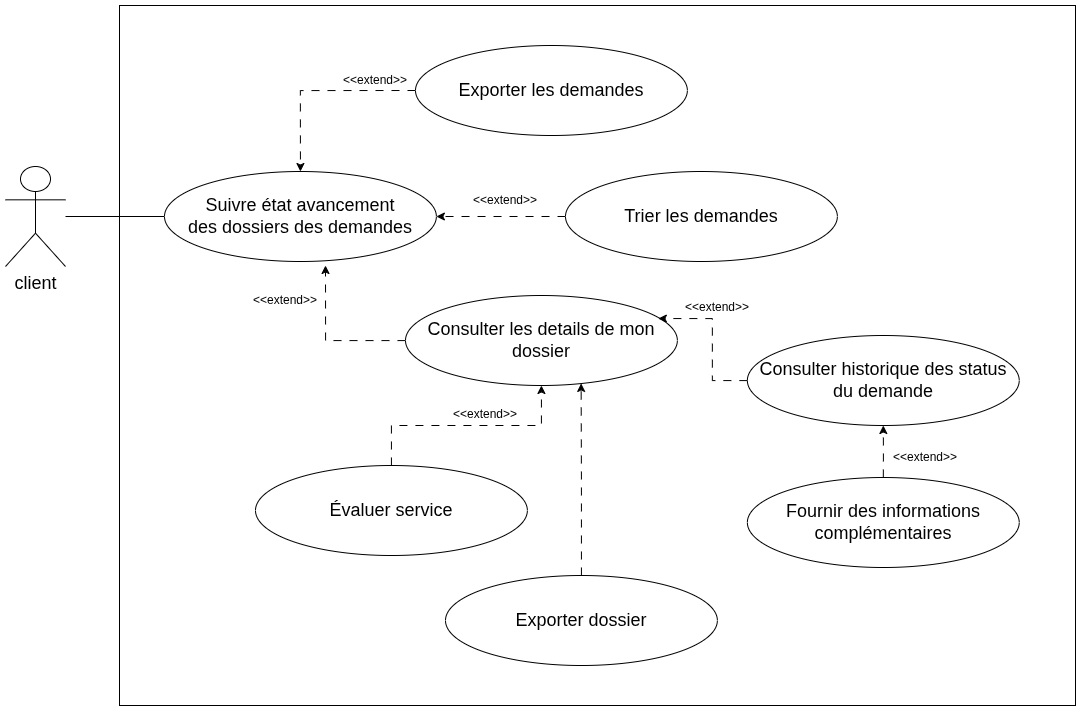
\includegraphics[width=15cm,height=10cm]{images/diagrammes/sprint3/cas-utilisation-sprint3-raff.drawio.png}
    \caption{Raffinement du cas d'utilisation « Suivre état avancement des dossiers des demandes »}
    \label{fig:cas-utilisation-sprint3-raff}
\end{figure}

\textbf{Description textuelle}


Une description détaillée du cas d’utilisation « Suivre état avancement des dossiers des demandes » est présentée dans le tableau~\ref{tab:uc-suivre-dossier}.

\begin{longtable}{|p{4cm}|p{12cm}|}
\hline

\rowcolor{gray!20}
\textbf{Champ} & \textbf{Description} \\ \hline
\endfirsthead

 

Nom & Consulter le détail de mon dossier \\ \hline

Acteur principal & Client e-Gouv \\ \hline

Objectif & Permettre au citoyen de consulter l’état d’avancement de sa demande administrative. \\ \hline

Pré-condition &
\begin{itemize}
    \item Le client est authentifié.
    \item Une demande de service a déjà été soumise.
\end{itemize}
\\ \hline

Scénario nominal &
\begin{enumerate}
    \item Le client accède à son espace personnel.
    \item Il consulte la liste de ses demandes.
    \item Il sélectionne une demande spécifique.
    \item Le système affiche les détails du dossier ainsi que son statut actuel.
    \item Le client peut consulter les étapes de traitement du dossier.
\end{enumerate}
\\ \hline

Scénario alternatif &
\begin{itemize}
    \item Si aucune demande n’existe, le système affiche un message informatif.
\end{itemize}
\\ \hline

Post-condition & Le client peut voir les informations et l’avancement de son dossier. \\ \hline

\caption{Description textuelle : Consulter le détail de mon dossier}
\label{tab:uc-suivre-dossier}

\end{longtable}


Une description détaillée du cas d’utilisation « Évaluer service » est présentée dans le tableau~\ref{tab:uc-evaluer-service}.

\begin{longtable}{|p{4cm}|p{12cm}|}
\hline

\rowcolor{gray!20}
\textbf{Champ} & \textbf{Description} \\ \hline
\endfirsthead

 

Nom & Évaluer service \\ \hline

Acteur principal & Client e-Gouv \\ \hline

Objectif & Permettre au client d’exprimer son niveau de satisfaction concernant un service administratif après le traitement de sa demande. \\ \hline

Pré-condition &
\begin{itemize}
    \item La demande de service est clôturée ou finalisée.
    \item Le client accède au détail de sa demande.
\end{itemize}
\\ \hline

Scénario nominal &
\begin{enumerate}
    \item Le client consulte une demande traitée.
    \item Il sélectionne l’option « Évaluer service ».
    \item Le système affiche un tableau d’évaluation de satisfaction.
    \item Le client écrit un commentaire et choisit un niveau de satisfaction :
    \begin{itemize}
        \item Très satisfaisant
        \item Satisfait
        \item Moyennement satisfait
        \item Peu satisfaisant
        \item Non satisfait
    \end{itemize}
    \item Le client valide son évaluation.
    \item Le système enregistre le niveau de satisfaction.
\end{enumerate}
\\ \hline

Scénario alternatif &
\begin{itemize}
    \item Si le client annule l’opération, aucune évaluation n’est enregistrée.
    \item Si une évaluation existe déjà, le système empêche une seconde soumission.
\end{itemize}
\\ \hline

Post-condition & L’évaluation du niveau de satisfaction du client est enregistrée et peut être exploitée à des fins statistiques et d’amélioration des services. \\ \hline

\caption{Description textuelle : Évaluer service}
\label{tab:uc-evaluer-service}

\end{longtable}


\subsection{Les diagrammes de séquences du cas d’utilisation « Suivre état avancement des dossiers des demandes »}

Dans cette section, nous avons choisi de présenter certains diagrammes de séquence parmi ceux définis lors de l’étape de raffinement du sprint « Suivi des demandes ». Ce choix permet de mettre en évidence les interactions les plus significatives du système, notamment la consultation du dossier, l’évaluation du service, l’exportation des demandes ainsi que la fourniture d’informations complémentaires. Ces diagrammes illustrent les principaux échanges entre le citoyen et le système dans le cadre du traitement des demandes administratives.

\noindent  \textbf{Présentation des diagrammes de séquences :}

% Consulter
 Comme présenté dans la figure~\ref{fig:consulter-form-seq} ce diagramme de séquence illustre le processus de suivi du  dossier de demande. Il décrit les différentes interactions permettant au citoyen de consulter les détails d’un dossier, son statut actuel ainsi que les différentes étapes de traitement effectuées par l’administration.

\begin{figure}[H]
    \centering
    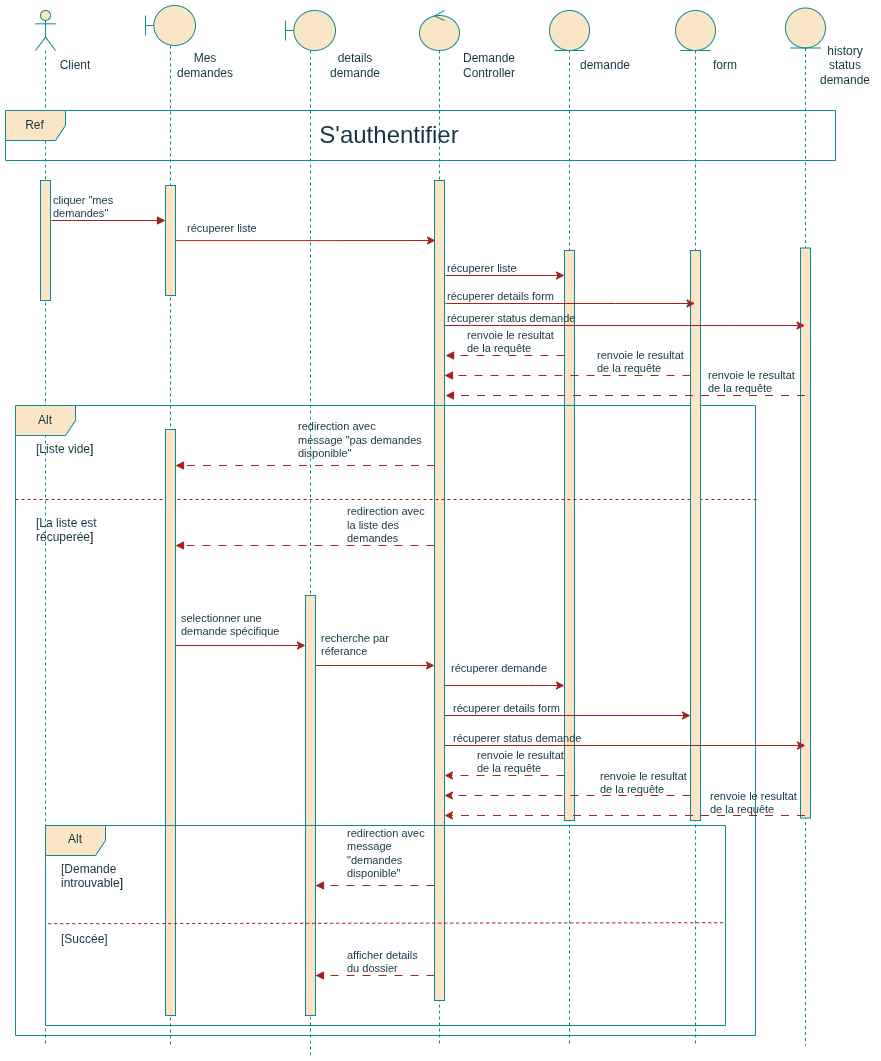
\includegraphics[width=15cm,height=16cm]{images/diagrammes/sprint3/consulter-demandes.drawio.png}
    \caption{Diagramme de séquence - Consulter le détails de mon dossier}
    \label{fig:consulter-form-seq}
\end{figure}


% evaluer
 Comme présenté dans la figure~\ref{fig:evaluer-seq} ce diagramme de séquence présente le processus d’évaluation d’un service administratif après le traitement d’une demande. Il met en évidence les échanges permettant au citoyen de sélectionner un niveau de satisfaction afin de partager son retour d’expérience sur le service reçu.

\begin{figure}[H]
    \centering
    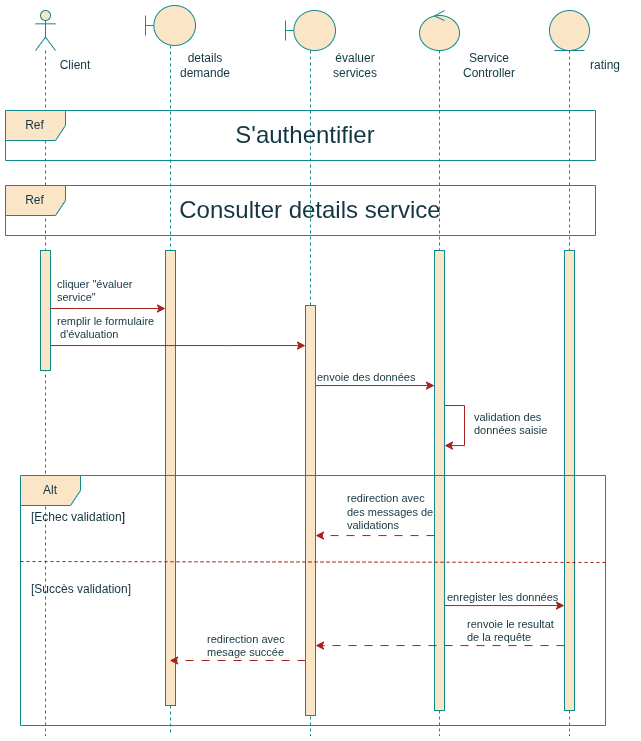
\includegraphics[width=18cm,height=16cm]{images/diagrammes/sprint3/Evaluer-demande.drawio.png}
    \caption{Diagramme de séquence - Évaluer service}
    \label{fig:evaluer-seq}
\end{figure}


\subsection{Réalisation du sprint 3 : « Suivre état avancement des dossiers des demandes »}

Dans cette section nous présentons certaines interfaces représentatives de la réalisation du sprint « Suivi des demandes », afin d’illustrer les principales fonctionnalités mises en œuvre. Ce choix met en évidence les écrans les plus significatifs du système, notamment la consultation des dossiers, l’évaluation des services, l’exportation des informations ainsi que la fourniture de données complémentaires. Ces captures permettent de visualiser concrètement l’interaction du citoyen avec le système tout au long du traitement de ses demandes administratives.

\noindent \textbf{Présentation des interfaces :}

 L’interface présentée dans la figure~\ref{fig:consult-detail-dossier} permet au citoyen de consulter les détails de ses dossiers administratifs. Elle offre une visibilité sur les informations associées à la demande, le statut actuel ainsi que les différentes actions disponibles liées au traitement du dossier.

 


\begin{figure}[H]
    \centering
    \fbox{%
        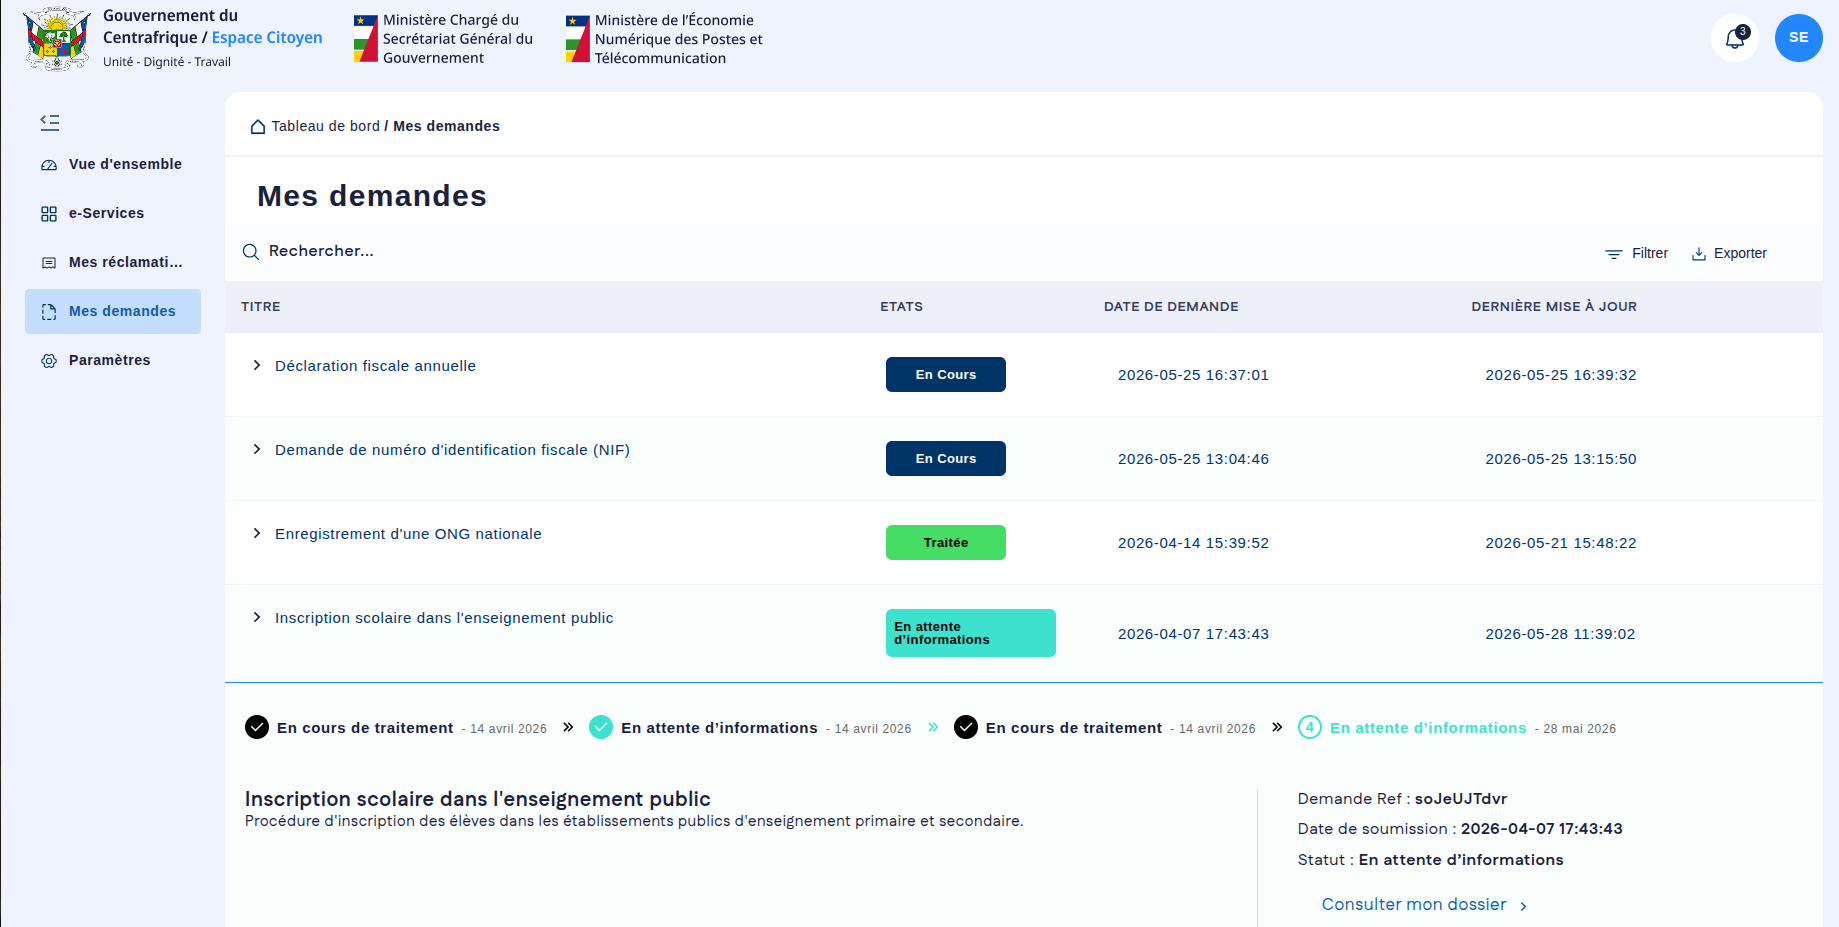
\includegraphics[width=0.95\textwidth]{images/realisation/sprint3/Capture-list.png}
    }
    \caption{Consultation du détail d’un dossier}
    \label{fig:consult-detail-dossier}
\end{figure}







 
 L’interface présenté dans la figure~\ref{fig:evaluer-service} illustre le mécanisme d’évaluation d’un service administratif. Une fois la demande traitée, le citoyen peut exprimer son niveau de satisfaction afin de contribuer à l’amélioration continue de la qualité des services publics.

 

\begin{figure}[H]
    \centering
    \fbox{%
        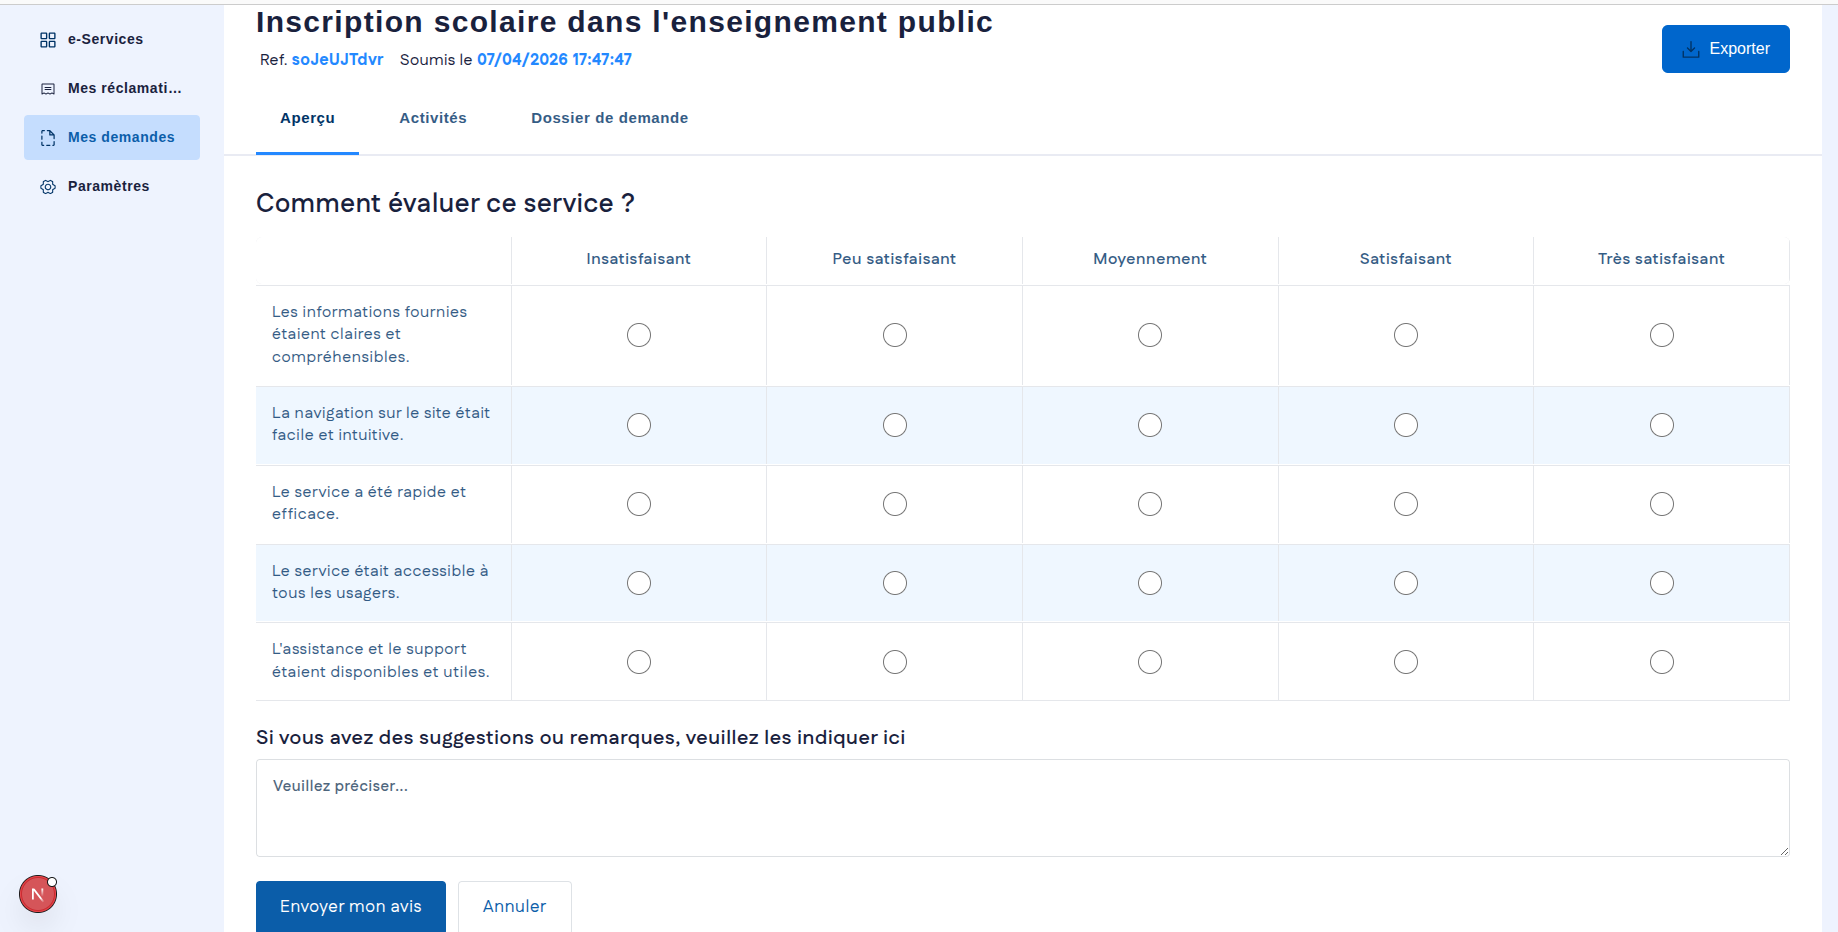
\includegraphics[width=0.95\textwidth]{images/realisation/sprint3/Capture-evaluer.png}
    }
    \caption{Évaluation d’un service}
    \label{fig:evaluer-service}
\end{figure}

 L’interface présenté dans la figure~\ref{fig:exporter-dossier},  présente le résultat d’exportation des informations du dossier administratif. Cette fonctionnalité facilite la conservation, le partage ou l’impression des données relatives à la demande.

\begin{figure}[H]
    \centering
    \fbox{%
        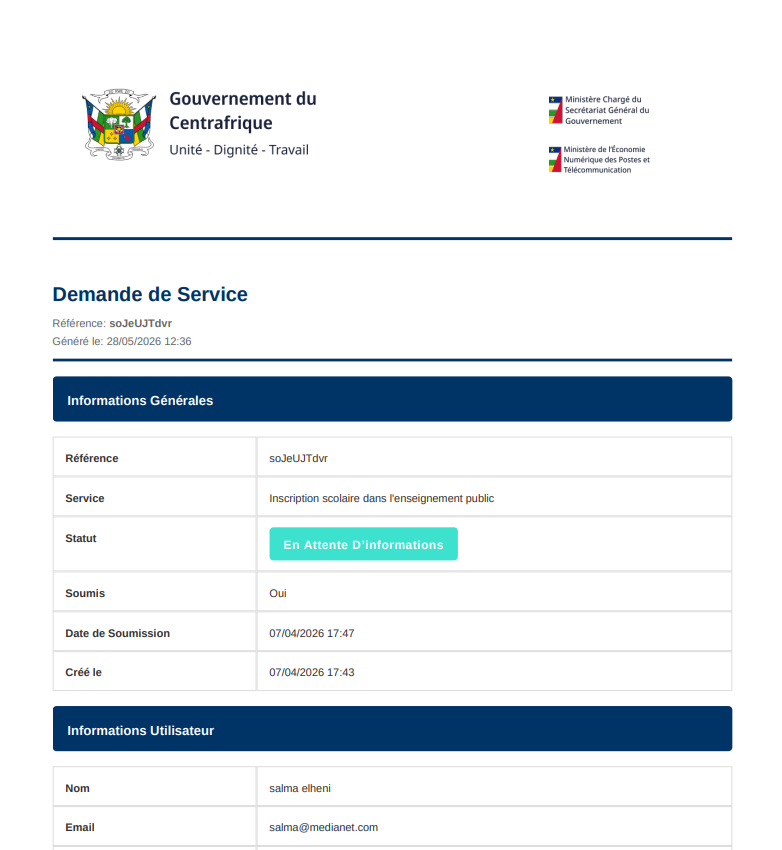
\includegraphics[width=0.95\textwidth]{images/realisation/sprint3/Capture-export.png}
    }
    \caption{Exportation d’un dossier}
    \label{fig:exporter-dossier}
\end{figure}


 L’interface présenté dans la figure~\ref{fig:info-complementaire},  présente le processus d’ajout d’informations complémentaires demandées par l’administration. Le citoyen peut fournir des documents ou des informations supplémentaires afin de compléter le traitement de son dossier.

\begin{figure}[H]
    \centering
    \fbox{%
        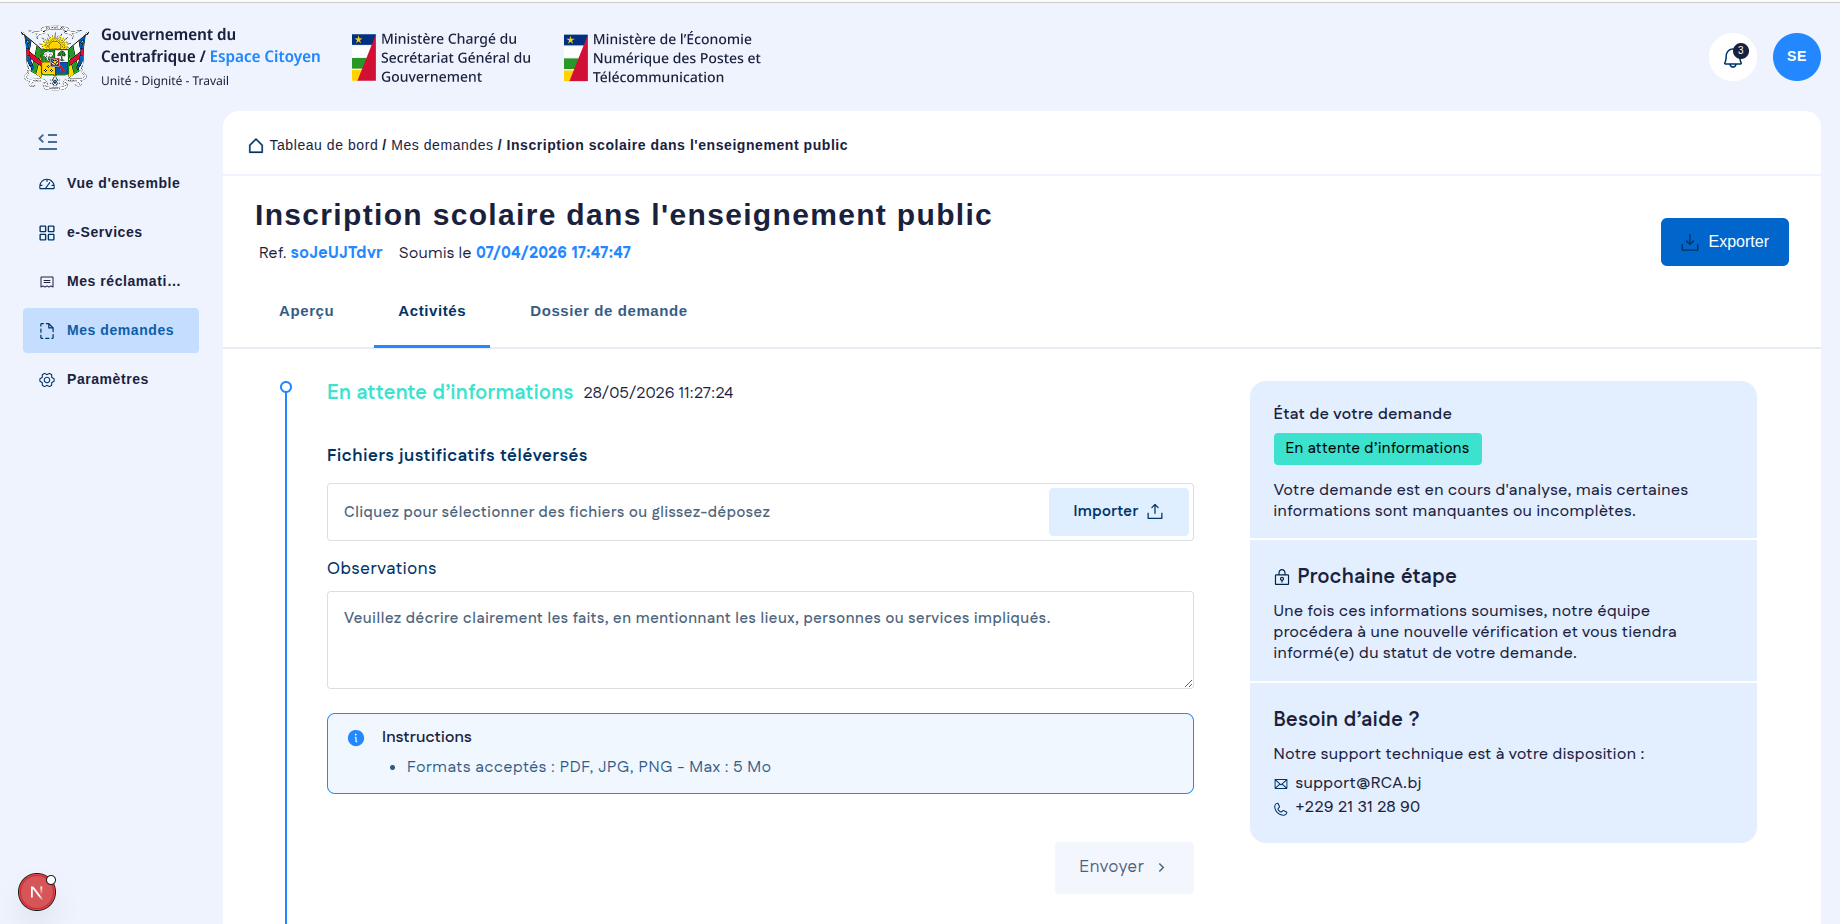
\includegraphics[width=0.95\textwidth]{images/realisation/sprint3/Capture-complemantary.png}
    }
    \caption{Fourniture d’informations complémentaires}
    \label{fig:info-complementaire}
\end{figure}


\subsection{Revue du Sprint 3}

A l'issue du Sprint 3 l'ensemble des user stories planifiées ont été développées et validées, comme présenté dans le tableau~\ref{tab:revue-sprint3}.

\begin{longtable}{|c|p{9cm}|c|}
\hline
\rowcolor{orange!30}
\textbf{ID} & \textbf{User Story} & \textbf{Statut} \\ \hline
US16 & Déposer une demande de service en ligne & \textcolor{green!60!black}{Terminé} \\ \hline
US17 & Suivre l'état d'avancement de mes dossiers & \textcolor{green!60!black}{Terminé} \\ \hline
US18 & Évaluer un service après traitement & \textcolor{green!60!black}{Terminé} \\ \hline
US19 & Consulter mon tableau de bord & \textcolor{green!60!black}{Terminé} \\ \hline
US20 & Modifier mon profil (Client) & \textcolor{green!60!black}{Terminé} \\ \hline
US11 & Personnaliser les étapes de traitement des demandes & \textcolor{green!60!black}{Terminé} \\ \hline
US24 & Gérer les demandes de service (Admin Institutionnel) & \textcolor{green!60!black}{Terminé} \\ \hline
\caption{Revue du Sprint 3}
\label{tab:revue-sprint3}
\end{longtable}





\section{Conclusion}

Cette première release a permis de mettre en place les fondations du système à travers la gestion des utilisateurs et des structures administratives, la configuration du catalogue de services ainsi que la dématérialisation et le suivi des demandes en ligne.

Elle constitue une étape clé dans la mise en œuvre de la plateforme e-Gouvernement, en améliorant l’accessibilité et la gestion des services administratifs pour les citoyens et les administrateurs.
 
